\documentclass[aps,prx,onecolumn,superscriptaddress,longbibliography]{revtex4-2}
\usepackage[utf8]{inputenc}
\usepackage[T1]{fontenc}
\usepackage{amsmath,amssymb,graphicx,booktabs,newunicodechar,url}
\newcommand{\tabrr}{\raggedright\let\\\tabularnewline}
\newunicodechar{−}{\ensuremath{-}}\newunicodechar{×}{\ensuremath{\times}}\newunicodechar{≤}{\ensuremath{\le}}
\newunicodechar{≥}{\ensuremath{\ge}}\newunicodechar{≈}{\ensuremath{\approx}}\newunicodechar{±}{\ensuremath{\pm}}
\newunicodechar{∂}{\ensuremath{\partial}}\newunicodechar{Σ}{\ensuremath{\Sigma}}\newunicodechar{Δ}{\ensuremath{\Delta}}
\newunicodechar{κ}{\ensuremath{\kappa}}\newunicodechar{ρ}{\ensuremath{\rho}}\newunicodechar{θ}{\ensuremath{\theta}}
\newunicodechar{λ}{\ensuremath{\lambda}}\newunicodechar{ν}{\ensuremath{\nu}}\newunicodechar{σ}{\ensuremath{\sigma}}
\newunicodechar{β}{\ensuremath{\beta}}\newunicodechar{ε}{\ensuremath{\varepsilon}}\newunicodechar{φ}{\ensuremath{\varphi}}
\newunicodechar{μ}{\ensuremath{\mu}}\newunicodechar{τ}{\ensuremath{\tau}}\newunicodechar{χ}{\ensuremath{\chi}}\newunicodechar{₂}{\ensuremath{_{2}}}\newunicodechar{α}{\ensuremath{\alpha}}\newunicodechar{√}{\ensuremath{\surd}}
\newunicodechar{ḡ}{\ensuremath{\bar{g}}}\newunicodechar{…}{\ldots}\newunicodechar{→}{\ensuremath{\to}}
\newunicodechar{Π}{\ensuremath{\Pi}}\newunicodechar{∞}{\ensuremath{\infty}}\newunicodechar{⁻}{\ensuremath{^{-}}}
\newunicodechar{⁹}{\ensuremath{^{9}}}\newunicodechar{¹}{\ensuremath{^{1}}}\newunicodechar{’}{'}\newunicodechar{–}{--}\newunicodechar{—}{---}\newunicodechar{′}{\ensuremath{'}}
\newunicodechar{²}{\ensuremath{^{2}}}\newunicodechar{₀}{\ensuremath{_{0}}}\newunicodechar{₁}{\ensuremath{_{1}}}
\providecommand{\texorpdfstring}[2]{#1}
\providecommand{\tightlist}{\setlength{\itemsep}{0pt}\setlength{\parskip}{0pt}}
\begin{document}
\title{A first-order prediction from unpenalized samples of how a repetition penalty changes switching into and out of repetitive text}
\author{Chisa Honda}
\email{chichichi2001@gmail.com}
\affiliation{Independent researcher}
\begin{abstract}
A repetition penalty acts on a language model at every sampling step, and the distribution is renormalized each time. We find that its effect on how generated text switches into and out of repetitive stretches follows a first-order prediction computed from samples generated without the penalty. This held at penalties that changed the ratio of the entry and exit rates about threefold. For an additive penalty \(h\) on repeat candidates (tokens that have previously followed the current last two tokens), the derivative of a text's log-probability at \(h\) = 0 is \((N-Q)/T\). Here \(N\) counts the candidates chosen, \(Q\) sums over steps the probability of choosing one, and \(T\) is the temperature. In a replication registered in advance, on new news articles and seven open base models, we divided the realized change in the log ratio of the rates by the first-order prediction. The median was 1.04, inside the registered range of 0.8 to 1.25. The derivative came from the unpenalized runs of the same test, so this shows that the response is still first order at these penalties. Differences between the models could not be distinguished from sampling noise. Reweighting the same unpenalized samples by their exact probability ratios could not determine the change, because the variance of the log-weights grows with the length of the text. In the same runs, the compensator \(Q\) cancels about 99\% of the response to reweighting whole texts. The widely used multiplicative penalty followed the prediction only at the weakest strengths common in practice, and the temperature that the penalties were designed to move was not controlled model by model.
\end{abstract}
\maketitle

\section{Introduction}

Language models that sample one token at a time sometimes fall into loops, repeating a phrase or a sentence until the end of the output. This problem is old and persists in current systems \cite{1904.09751,2012.14660,2206.02369,2310.10226,2512.12895}. Repetition reinforces itself: the more often a phrase has been repeated, the more likely it is to be repeated again \cite{2206.02369}. It has been addressed by adaptive sampling \cite{2007.14966}, by training objectives that discourage it \cite{1908.04319} and, most often, by penalizing at inference the tokens that would repeat earlier text \cite{1909.05858}. In a production setting such a penalty removed only some kinds of repetition \cite{2512.04419}, and penalties derived from a model of expected frequencies have also been proposed \cite{2607.22694}. How strong a penalty must be is usually found by trial.

Sampling at temperature \(T\) draws each token with probability proportional to \(\exp(z/T)\), where z is the logit of that token. Several studies have described generated text in the language of statistical physics, with phases and transitions as the temperature changes \cite{2406.05335,2503.06330,2405.17088,2606.06238}. In small models, repetitive structure has been reported to appear only in a low-temperature ordered phase \cite{2406.05335,2503.06330}. These works describe generated text but do not predict how an intervention such as a penalty acts. A natural shortcut would treat the penalty as an energy per chosen candidate in a two-state Boltzmann system. Appendix H shows why this shortcut is not a reliable guide.

The Boltzmann form holds for each step and not for the text as a whole. At \(T\) = 1 the probability of a text is \(\exp(-U(x))\), with \(U\) the sum over its tokens of \(-\log p\) at \(T\) = 1. At any other temperature, or with any change to the logits, the distribution is normalized afresh at every step \cite{2503.21929}. The probability of a text is then, in general, not \(\exp(-U(x)/T)/Z(T)\) for an additive energy \(U\) that is independent of \(T\). The response of such a process to a change in its transition probabilities is given exactly by a likelihood-ratio, or score-function, formula \cite{Glynn1990,Williams1992,WarrenAllen2012}. We use this formula to predict the effect of a penalty from unpenalized samples, and test the predictions after registering them. With the same formula we measure how much of a whole-text, Boltzmann-like response survives step-wise normalization. This explains why a penalty's effect is much smaller than that response. We also locate where in a text a penalty acts.

In sequence labeling, locally normalized models can be biased in ways that globally normalized ones are not, a problem known as label bias \cite{LaffertyEtAl2001,AndorEtAl2016,WisemanRush2016}. In statistical physics, reweighting whole trajectories gives tilted ensembles, which can be written step by step as Doob transforms \cite{GarrahanEtAl2009,JackSollich2010,ChetriteTouchette2015}. Language-model decoding has been steered by estimates of a future reward or attribute \cite{YangKlein2021,ZhaoEtAl2024}, and Kempton and Burrell described how local normalization distorts temperature and truncation relative to a global Boltzmann form \cite{2503.21929}. Here we bring these ideas to a repetition penalty and test the resulting prediction prospectively, on one statistic of the switching between repetitive and ordinary text.

\section{Setup}

We sampled continuations of news articles published after the models were released, from nine open base models with 0.4 to 7.6 billion parameters (Table I; Appendix A). Sampling was plain softmax at temperatures between 0.19 and 0.90. Each test used seven temperatures per model, centered on a design temperature chosen for that model (Sec. IV B), with no truncation such as top-k or top-p.~End-of-sequence and padding tokens were excluded, so that no continuation could end early, and all probabilities below, including the candidate probability \(q_{t}\) defined next, refer to this masked distribution. Each prompt was the first 64 tokens of an article, and the model generated four continuations of 512 tokens from it. We call one round of computing the next-token logits, adjusting them, normalizing them and sampling one token a step.

\textbf{Repeats and penalties.} A sampled token is a repeat if the four tokens ending with it occurred earlier in the same continuation, that is, if it ends a repeated 4-gram. The penalty acts on a slightly broader set. At step \(t\) the repeat candidates are the tokens that have previously followed the current last two tokens, in the prompt or the continuation. We write \(c_{t}\) = 1 if the sampled token is a candidate and \(c_{t}\) = 0 otherwise, and \(q_{t}\) for the total probability that the model, at temperature \(T\) and without the penalty, assigns to the candidates. Repeats define the states below and candidates define the penalty, so that the definition of the states does not depend on the penalty. The additive penalty adds \(h\) to the logits of the candidates before division by \(T\), so that \(h\) \textless{} 0 discourages repetition. This additive penalty is not an option in common libraries. It acts like a logit bias on a set that depends on the context, and we use it because its exact score has the simplest form. A widely used multiplicative penalty, implemented as repetition\_penalty in common libraries, acts on a third set, all tokens that have appeared earlier. Prior to division by \(T\), it divides their positive logits by θ and multiplies their negative logits by θ \cite{1909.05858,1910.03771}.

\textbf{Two states and the crossover temperature.} Repeats cluster into long stretches separated by ordinary text. We label each step as repetitive or ordinary from the fraction of repeats in a 32-token window around the step, 16 tokens before it and 15 after. The label has hysteresis: a step enters the repetitive state when the fraction reaches 1/2 and leaves it when the fraction falls below 1/4 (Appendix A). Each label therefore uses up to 15 later tokens. At each temperature we count switches into the repetitive state per ordinary step, the entry rate, and switches out of it per repetitive step, the exit rate. Their ratio, \(K\) = entry rate/exit rate, measures the balance between the two states. We call the temperature at which \(K\) = 1 the crossover temperature \(T_{\times}\). Near \(T_{\times}\), \(\ln K\) is close to linear in 1/\(T\), as in a van 't Hoff plot, and over wider ranges it curves. An analysis uses a temperature only if both kinds of switch occurred there at least ten times in every arm being compared. We call these the usable temperatures.

The two states are a labeling, not distinct phases. The windowed repeat fraction has peaks near zero and at one, but it did not meet a bimodality criterion we had fixed in advance (Appendix F1). \(K\) is also not the rate ratio of a stationary two-state Markov chain. The balance drifts towards repetition along a text, and repetitive stretches become harder to leave the longer they last (Appendix F2). We use \(K\) as a summary of switching statistics, averaged over positions and over stretches of different duration. \(T_{\times}\) depends on the labeling and on the length of the continuation, so we compare it only within a fixed labeling and length.

\section{Theory}

\textbf{A. Score of a penalized text.} A continuation \(x=(x_1,\ldots,x_L)\) has probability \(P_h(x)=\prod_t p_t^h(x_t\mid x_{<t})\). For the additive penalty, the derivative of \(\log p_t^h(x_t)\) at \(h\) = 0 is \((c_t-q_t)/T\). Summing over steps,

\begin{equation}\left.\frac{\partial \log P_h(x)}{\partial h}\right|_{h=0}=\frac{N-Q}{T},\qquad N=\sum_t c_t,\quad Q=\sum_t q_t.\end{equation}

Here the length \(L\) is fixed, with no early stopping. The identity also holds with a bounded stopping time, such as stopping at an end-of-sequence token or at a maximum length, whichever comes first, but we did not use one. \(N\) is the number of candidates chosen. \(Q\) is its compensator, the sum of the probabilities of choosing a candidate given the text so far: each \(q_{t}\) is fixed by the text before step \(t\), and \(N\) − \(Q\) has mean zero. For any statistic \(O\) of the text that does not itself depend on \(h\), the response at \(h\) = 0 is therefore

\begin{equation}\frac{\partial E[O]}{\partial h}=\frac{\mathrm{Cov}(O,N)}{T}-\frac{\mathrm{Cov}(O,Q)}{T}.\end{equation}

Applied to the four counts that define \(K\) (entries, exits, and ordinary and repetitive steps; Appendix A), this gives the exact derivative \(g(T)=\partial\ln K/\partial h\), where \(K\) is defined by ratios of expected counts (Appendix B). For the multiplicative penalty, with λ = \(\ln \theta\), \(c_{t}\) − \(q_{t}\) is replaced by \(a_t-E_t[a]\) (Appendix B). Here \(a\) is the derivative of a token's logit with respect to λ, and \(E_{t}\) the expectation under the step-\(t\) distribution.

\textbf{B. Step-wise penalty versus exponential tilting.} A penalty that acted on the text as a whole would instead reweight it. Reweighting each whole text by \(\exp(hN/T)\) and renormalizing is called exponential tilting in statistics; in statistical physics the result is a tilted ensemble of trajectories. It gives the response \(\mathrm{Cov}(O,N)/T\), the static susceptibility of the path ensemble. The step-wise response equals this tilted response minus \(\mathrm{Cov}(O,Q)/T\). To see what the difference means, write \(N-E[N]\) as the sum of updates of the expected final count, \(E[N\mid x_{\le t}]-E[N\mid x_{<t}]\). Each update is \(c_t-q_t\) plus \(\nu_t\). Here \(\nu_{t}\) is the change, on learning \(x_{t}\), in the expected number of candidates chosen after step \(t\), and it has mean zero given the earlier text. Summing over t gives \(N-E[N]=(N-Q)+\sum_t \nu_t\), so \(Q-E[Q]=\sum_t \nu_t\) and

\begin{equation}\mathrm{Cov}(O,Q)=\mathrm{Cov}\Big(O,\sum_t \nu_t\Big).\end{equation}

Exponential tilting also rewards each choice, or for \(h\) \textless{} 0 penalizes it, for the candidates it makes likely to be chosen later. Written step by step, the tilted ensemble is again an autoregressive process. Its step probabilities are multiplied by \(\exp(hc_t/T)\) and by the expected future factor \(E[\exp(hN_{>t}/T)\mid x_{\le t}]\), with \(N_{>t}\) the number of candidates chosen after step \(t\), and renormalized. This is a finite-horizon Doob transform \cite{JackSollich2010,ChetriteTouchette2015}. To first order in \(h\), after renormalization, the expected future factor adds \((h/T)\sum_t \nu_t\) to the log-weight of a text, a term that a step-wise penalty lacks. Entering a repetitive stretch makes many future repeats likely, so this is where we expect the two to differ most. Writing \(g_{N}\) for the response of \(\ln K\) under exponential tilting by \(\exp(hN/T)\), we call \(s_{\mathrm{pen}}\) = \(g\)/\(g_{N}\) the fraction of the tilted response that survives step-wise normalization.

\textbf{C. An equilibrium shortcut and temperature.} A two-state Boltzmann model that treats the penalty as an energy per chosen candidate also predicts the response from unpenalized samples. It needs an energy for each step, which the sampler does not define, and its prediction changes with that choice; the identities above do not. Changing the temperature is also a step-wise change, with its own compensator. Both are developed in Appendix H.

\section{Results}

\subsection{Two states and the crossover temperature}

Consider a temperature where both kinds of stretch are common. There, the fraction of repeats in a 32-token window has a high peak near zero, a narrow peak at exactly one and a shallow trough in between (Fig. 1b). Most outputs switch between the two kinds at least once. In the repetitive state the models chose a repeat candidate at almost every step, and in the ordinary state at about one step in five (Appendix F1).

The crossover temperature lies between 0.44 and 0.66 for the nine models (Fig. 1c; Table I).

\begin{figure}
\centering
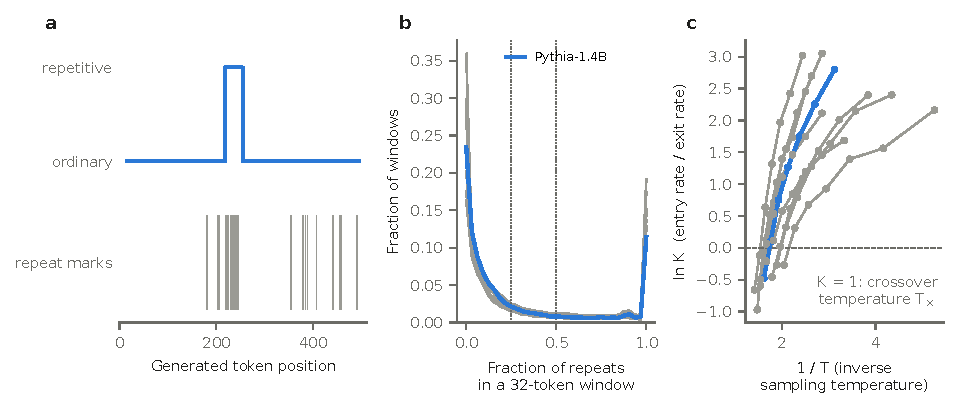
\includegraphics[width=\linewidth]{figures/fig1}
\caption{\textbf{Generated text alternates between repetitive and ordinary stretches.} (a), Repeat marks (grey ticks) and labeled state (line; up, repetitive) along one unpenalized continuation of Pythia-1.4B at $T$ = 0.62, chosen as the first output with two to six switches. (b), Distribution of the fraction of repeats in a 32-token window at the test temperature closest to each model's crossover temperature, for unpenalized continuations of the 120 replication articles. Grey, eight models; blue, Pythia-1.4B. Dotted lines, the thresholds for leaving (1/4) and entering (1/2) the repetitive state. (c), $\ln K$, the log ratio of entry rate to exit rate, against inverse temperature for the same runs. The crossover temperature is where $\ln K$ = 0.}
\label{fig1}
\end{figure}

\subsection{Predicting a penalty before applying it}

Penalizing or favoring the repeat candidates moved \(T_{\times}\) in the direction of \(h\), roughly linearly (Fig. S1). Because the derivative of Sec. III A needs only unpenalized samples, unpenalized runs on 40 design articles suffice to predict the penalty \(h^*\) that should lower \(T_{\times}\) by 0.10. We call \(T^*\) = \(T_{\times}\) − 0.10 the design temperature. Before generating any penalized text for these tests, we fixed the procedure, the analysis code and the decision criterion in dated documents. The runs behind Fig. S1 were made earlier and were analyzed under their own registration, before their data were opened (Appendix F7). Each test compares the realized change in \(\ln K\) at \(h^*\) with the first-order prediction \(h^*\) \(g\)(\(T\)); both are summed over the usable temperatures before their ratio is taken. Of the two factors of the prediction, only \(h^*\) was fixed beforehand, while \(g\) came from the unpenalized runs of the same test. The test therefore asks whether the response is still first order at \(h^*\). We required the bootstrap interval of the median ratio over the seven smaller models, or of the mean over the two larger ones, to lie between 0.8 and 1.25.

The first test, on the 40 articles from which \(h^*\) had been computed, was inconclusive: its intervals at \(h^*\) and at 2\(h^*\) both reached just above 1.25 (Appendix F3). We then committed in advance to a single replication on 120 new articles, with the same rule and statistic. Its median ratio was 1.04 (95\% interval 0.98--1.15), inside the range (Fig. 2; Table I). A separate test of two 7-billion-parameter models gave a mean ratio of 0.96 (0.84--1.11). Pooling the first test and the replication, 160 articles, gave 1.09 (0.98--1.15). None of the registered decisions depended on the number of bootstrap resamples, the seed or the kind of interval (Appendix C). For comparison, the tilted response of Sec. IV C would give a ratio of about 0.01. Per-model intervals were too wide to decide each model: two of the seven intervals of the replication, and neither of those of the larger models, lay inside the range (Table I). In an exploratory analysis the differences between the seven ratios were no larger than the article sample alone would produce. A standard deviation of the true ratios across models above about 12\% was excluded (Appendix C). Nor were the per-model departures of the first test reproduced in the replication, except for Pythia-1.4B. Under eight other labelings of the states the interval of the median also stayed inside the range (Table F2).

A user would estimate the derivative before applying the penalty, on other text. In an exploratory analysis we therefore replaced the denominator by the prediction made at design time, \(h\bar{g}\) at every usable temperature. Here ḡ is the temperature-averaged \(g\) from the design articles, and both sets of articles were resampled (Appendix F4). The median ratio was 1.05 (0.93--1.20) for the smaller models, inside the range, while the test on the larger models did not decide. The median rule does not single out the model's own derivative. A ḡ averaged over the other six models also gave a median inside the range, and the accuracy per model of the two could not be distinguished. The first-order response also predicted the change in the fraction of steps marked as repeats, a quantity closer to what users measure. For the fraction in the last 64 steps alone the test was undecided (Appendix F4).

The same procedure predicted the divisor θ of the multiplicative penalty. At the predicted divisors the median ratio over seven models was 1.01, with its interval inside the range. The prediction still held with \(\ln \theta\) set to twice its predicted value, the test was inconclusive at four times, and the ratio fell below the range at eight times (Appendix F5). The confirmed divisors reach only the lower end of the values of 1.1 to 1.3 common in practice. For two instruction-tuned models the test was inconclusive for one and could not be run for the other.

The shift of \(T_{\times}\) itself, which the design targeted, was larger than intended. With \(T_{\times}\) located by a straight-line fit of \(\ln K\) against 1/\(T\), as in the design, its median was 1.3 times the intended shift in the smaller models. Locating each crossing by interpolation after the tests brought the median close to the target. Individual models, however, ranged from 0.5 to 2.4 times the intended shift, and no per-model interval lay inside the range (Appendix F6). In a check made after the tests, we found that the ordering of the models, though not the size of their departures, was already visible in the design data. The derivative at each model's crossover agreed to within a quarter with the slope of \(T_{\times}\) measured on the design runs. But \(h^*\) had been set with \(g\) averaged over the design temperatures, and where \(g\) changed with temperature, this average differed from its value at the crossover. For GPT-2-XL, which overshot most, the measured slope times \(h^*\) implied 1.6 times the intended shift, against 2.4 realized.

\begin{figure}
\centering
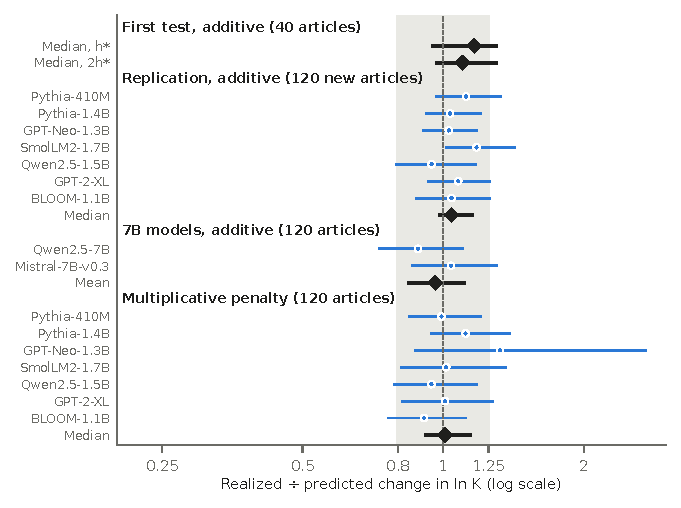
\includegraphics[width=\linewidth]{figures/fig2}
\caption{\textbf{Prospective tests.} Ratio of the realized change in $\ln K$ to the first-order prediction, with 95\% bootstrap intervals over articles, for each preregistered test. Circles, individual models. Diamonds, the test statistic (median or mean) with its interval. The multiplicative block is at the predicted divisor $\theta^*$; the stronger divisors and the instruction-tuned models are in Appendix F5. For the first test only the statistics are shown, for $h^*$ and 2$h^*$ (per-model values in Appendix F3). Grey band, the preregistered range 0.8–1.25. Logarithmic axis.}
\label{fig2}
\end{figure}

\begin{table}[htbp]
\centering
\small
\setlength{\tabcolsep}{6pt}
\caption{\textbf{Models and prospective tests.} Crossover temperature \(T_{\times}\): unpenalized, from the fit used for the prediction. \(h^*\): predicted additive penalty on the logits of repeat candidates (before division by temperature) that should lower \(T_{\times}\) by 0.10. Ratio: realized change in \(\ln K\) divided by the first-order prediction from the same test, both summed over the usable temperatures, with a 95\% bootstrap interval over articles (120 articles in each of these two tests). Design-only: the same realized change divided by the prediction made at design time (exploratory; intervals resample the design and the test articles). First seven models: preregistered replication. Last two models: preregistered test on 7-billion-parameter models. Decision band: 0.8--1.25 (median over the first seven models; mean over the last two). The lower ends shown as 0.80 are 0.796 (Qwen2.5-1.5B, ratio) and 0.799 (Pythia-410M, design-only), below 0.8.}
\label{tabI}
\begin{tabular}{@{}p{0.164\dimexpr\columnwidth-12\tabcolsep\relax}p{0.173\dimexpr\columnwidth-12\tabcolsep\relax}p{0.155\dimexpr\columnwidth-12\tabcolsep\relax}p{0.136\dimexpr\columnwidth-12\tabcolsep\relax}p{0.164\dimexpr\columnwidth-12\tabcolsep\relax}p{0.209\dimexpr\columnwidth-12\tabcolsep\relax}@{}}
\toprule
\tabrr Model & \tabrr Parameters (billions) & \tabrr \(T_{\times}\) & \tabrr \(h^*\) & \tabrr Ratio (95\% interval) & \tabrr Design-only ratio (95\% interval) \\
\midrule
\tabrr Pythia-410M & \tabrr 0.41 & \tabrr 0.60 & \tabrr −0.40 & \tabrr 1.12 (0.97--1.33) & \tabrr 0.96 (0.80--1.20) \\
\tabrr Pythia-1.4B & \tabrr 1.4 & \tabrr 0.57 & \tabrr −0.50 & \tabrr 1.03 (0.92--1.20) & \tabrr 1.06 (0.86--1.41) \\
\tabrr GPT-Neo-1.3B & \tabrr 1.3 & \tabrr 0.63 & \tabrr −0.39 & \tabrr 1.03 (0.91--1.18) & \tabrr 1.05 (0.89--1.28) \\
\tabrr SmolLM2-1.7B & \tabrr 1.7 & \tabrr 0.51 & \tabrr −0.53 & \tabrr 1.18 (1.02--1.42) & \tabrr 1.13 (0.92--1.41) \\
\tabrr Qwen2.5-1.5B & \tabrr 1.5 & \tabrr 0.60 & \tabrr −0.47 & \tabrr 0.94 (0.80--1.17) & \tabrr 1.02 (0.75--1.54) \\
\tabrr GPT-2-XL & \tabrr 1.6 & \tabrr 0.48 & \tabrr −0.79 & \tabrr 1.08 (0.93--1.26) & \tabrr 1.29 (1.05--1.67) \\
\tabrr BLOOM-1.1B & \tabrr 1.1 & \tabrr 0.66 & \tabrr −0.37 & \tabrr 1.04 (0.88--1.26) & \tabrr 0.86 (0.68--1.15) \\
\tabrr Median (first seven) & \tabrr & & \tabrr & 1.04 (0.98--1.15) & \tabrr 1.05 (0.93--1.20) \\
\tabrr Qwen2.5-7B & \tabrr 7.6 & \tabrr 0.55 & \tabrr −0.67 & \tabrr 0.88 (0.73--1.10) & \tabrr 1.19 (0.90--1.73) \\
\tabrr Mistral-7B-v0.3 & \tabrr 7.2 & \tabrr 0.44 & \tabrr −0.35 & \tabrr 1.04 (0.86--1.30) & \tabrr 0.96 (0.76--1.24) \\
\tabrr Mean (last two) & \tabrr & & \tabrr & 0.96 (0.84--1.11) & \tabrr 1.07 (0.91--1.35) \\
\bottomrule
\end{tabular}
\end{table}


\subsection{Step-wise normalization cancels almost all of the tilted response}

Table II compares each step-wise response with the response under exponential tilting, on the unpenalized runs of the replication and of the test on the larger models. For the penalty, the step-wise response of \(\ln K\) was between 0.7\% and 1.5\% of the tilted response (\(s_{\mathrm{pen}}\)). For \(\ln K\), the compensator term thus cancels about 99\% of the tilted term. Both responses are first-order quantities at \(h\) = 0. Nearly all of the covariance of the switching counts with \(N\) comes through the candidates that each choice makes likely to be chosen later, and \(Q\) carries the same expected later choices (Sec. III B).

The surviving fraction is of the order of one over the time scale of the switching. With \(k_{01}\) and \(k_{10}\) the entry and exit rates per step, the relaxation time τ = 1/(\(k_{01}\) + \(k_{10}\)) was 90 to 146 steps, and \(s_{\mathrm{pen}}\) τ lay between 0.9 and 1.5 for the nine models (Table II). A whole-text reweighting credits each choice with the later choices it makes likely, which may extend over about one relaxation time, while the step-wise penalty keeps only the choice itself. We did not test this reading. Across the smaller models \(s_{\mathrm{pen}}\) and 1/τ were not ordered alike. The criterion we had fixed beforehand, a coefficient of variation of \(s_{\mathrm{pen}}\) τ below 0.3, would have been met even if the two were unrelated (Appendix F8). τ also depends on the labeling, and the states do not form a stationary Markov chain (Appendix F2). These fractions use covariances within articles; pooling the numerator over articles, as in the tests, changes them little (Appendix F8). For the first 256 tokens \(s_{\mathrm{pen}}\) was 1.8\%, consistent with fewer later steps following each choice (Appendices B and F8). All of these are exploratory.

\begin{table}[htbp]
\centering
\small
\setlength{\tabcolsep}{6pt}
\caption{\textbf{Fraction of the tilted response that survives step-wise normalization, and the switching time.} \(s_{\mathrm{pen}}\): the step-wise response of \(\ln K\) to the penalty as a percentage of its response to exponential tilting by \(\exp(hN/T)\), summed over the usable temperatures. τ: median over the usable temperatures of 1/(\(k_{01}\) + \(k_{10}\)), in steps, with \(k_{01}\) and \(k_{10}\) the entry and exit rates per step. Unpenalized runs on the 120 articles of the replication (smaller models) and of the test on the larger models; for the larger models \(s_{\mathrm{pen}}\) τ uses \(s_{\mathrm{pen}}\) = 0.68\%. The temperature analogue, which depends on the energy assigned to a step, is in Appendix H.}
\label{tabII}
\begin{tabular}{@{}llll@{}}
\toprule
Model & \(s_{\mathrm{pen}}\) (\%) & τ (steps) & \(s_{\mathrm{pen}}\) τ \\
\midrule
Pythia-410M & 1.3 & 97 & 1.25 \\
Pythia-1.4B & 1.3 & 101 & 1.35 \\
GPT-Neo-1.3B & 1.5 & 103 & 1.50 \\
SmolLM2-1.7B & 1.1 & 101 & 1.08 \\
Qwen2.5-1.5B & 0.8 & 122 & 0.99 \\
GPT-2-XL & 1.1 & 90 & 1.01 \\
BLOOM-1.1B & 1.2 & 108 & 1.25 \\
Qwen2.5-7B & 0.7 & 146 & 0.99 \\
Mistral-7B-v0.3 & 0.7 & 134 & 0.91 \\
\bottomrule
\end{tabular}
\end{table}


\subsection{Where the penalty acts}

Each step contributes \((c_t-q_t)/T\) to the score, a term whose variance given the earlier text is \(q_{t}\)(1 − \(q_{t}\))/T². Steps where the model chooses a candidate with probability \(q_{t}\) above 0.9 make up more than four-fifths of the steps with repeat candidates but carry only about a fifth of the predicted response. Steps with \(q_{t}\) between 0.1 and 0.9 make up about a tenth of those steps but carry about four-fifths of the response, close to their share of the variance (Fig. 3a). Proportionality to the variance is not implied by the form of the score; it holds if one unit of \(c_{t}\) − \(q_{t}\) moves \(\ln K\) about equally at every step. For the steps with \(q_{t}\) between 0.1 and 0.9, the share of the response divided by the share of the variance had a median of 0.96 (0.91--0.98), inside the range 0.8--1.25 fixed beforehand but slightly below one (exploratory; Table C1).

The penalty acts at both ends of a repetitive stretch. About half of the change in \(\ln K\) came from a lower entry rate and half from a higher exit rate, in the smaller and the larger models alike (Fig. 3b). The derivative predicted this split less well than the total. It put slightly more of the response on the exit rate than was measured, and the interval of the difference excluded zero for two of the nine models (Appendix F10).

\begin{figure}
\centering
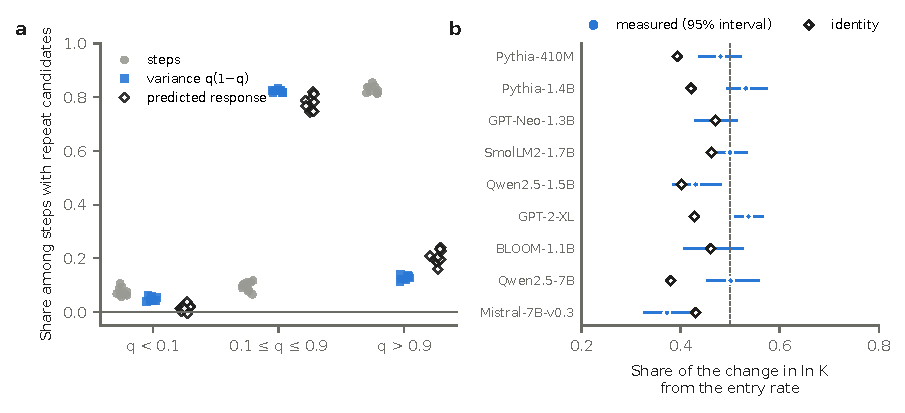
\includegraphics[width=\linewidth]{figures/fig3}
\caption{\textbf{Where the penalty acts.} (a), For steps with repeat candidates, split by the model's probability $q_{t}$ of choosing one (below 0.1, 0.1–0.9, above 0.9): share of the steps, share of the variance Σ $q_{t}$(1 − $q_{t}$) and share of the predicted response, for the nine models at the test temperatures. (b), Share of the realized change in $\ln K$ that comes from the change in entry rate (blue, 95\% interval) and the share predicted by the derivative (open diamonds). The rest comes from the exit rate. The interval shown is that of the measured share alone; the difference between the two shares, with both uncertainties, is in Appendix F10.}
\label{fig3}
\end{figure}

\section{Discussion}

For one statistic of the switching between repetitive and ordinary text, a first-order prediction computed from unpenalized samples matched the realized change at penalties large enough to move \(T_{\times}\). This held for the median of seven models, whose differences were within sampling noise, and the prediction also carried over to the fraction of repeats. In the registered tests the derivative came from the same runs. A prediction made from separate design articles also fell inside the range for the smaller models but did not decide for the two larger ones. The median rule could not tell the model's own derivative from one averaged over other models. The prediction depends on the signed difference between each candidate indicator \(c_{t}\) and the model's probability \(q_{t}\) of choosing a candidate, not on the number of candidates chosen alone. The compensator \(Q\) plays the role of the escape-rate term in the likelihood-ratio response of jump processes \cite{0902.3955,2005.10503}.

The first-order prediction held, for the median over models, at penalties with \textbar{}\(h^*\)\textbar/\(T^*\) between 0.67 and 2.1. Reweighting the 480 unpenalized continuations at each temperature by their exact probability ratios could not determine the change at these penalties. Only 5 to 18 effective samples remained, and the median ratio of the realized change to the reweighted estimate was 1.13 (0.84--2.08), with the wrong sign for GPT-2-XL (Appendix D). The variance of the log-weight grows with the length of the text, as (h/T)² \(\Sigma_{t}\) \(q_{t}\)(1 − \(q_{t}\)) to second order. \(\ln K\) is instead built from counts summed over many steps and texts, each of which a single choice changes only slightly. Whether a first-order prediction holds depends on this second scale, so the failure of reweighting does not by itself measure how far the response is from linear.

A natural shortcut, an equilibrium two-state model that treats the penalty as an energy, depends on the energy assigned to a step (Appendix H). Judged by the same statistic as the first-order prediction, with \(-\log p_t\) at \(T\) = 1 as the energy, its median ratio was 0.69 (0.64--0.72). With the negative logit \(-z\)\_t as the energy it predicted the wrong sign for two models.

The derivative of Sec. III A applies to any small shift added to the logits of a set of tokens, such as logit biases and watermarking biases \cite{2301.10226}. It also carries over to truncated sampling such as min-p \cite{2407.01082} or top-p \cite{1904.09751} if \(q_{t}\) is taken within the truncated set and the set does not change (Appendix G). We tested only the two repetition penalties, without truncation. Locating \(T_{\times}\) required unpenalized runs at several temperatures. For a single penalty, the score-based estimate of the derivative was about twice as noisy as a finite difference between two penalized arms with shared random numbers (Appendix F4). The approach pays off when many changes are evaluated from the same runs.

All prospective tests used English news articles, base models of up to 7.6 billion parameters and one family of labelings, with sampling rather than greedy or beam decoding, to which the score does not apply. Texts had 512 tokens, without truncation and with the end-of-sequence token masked; runs on novels, scientific papers and code are in Appendix F9. The widely used presence and frequency penalties were not tested, and the multiplicative penalty was confirmed only at the lowest strengths used in practice. Because the tests estimated the derivative from their own unpenalized runs, they test whether the response is first order at \(h^*\). Most point estimates lay slightly above one, 1.09 when the first test and the replication were pooled. The second-order term that could explain this can be estimated from the same samples, but it was not determined at this sample size (Appendix F3). The confirmation rests on one replication after an inconclusive first test and on one test of two larger models. The additive, multiplicative and larger-model tests share the same 120 articles, and the bootstrap intervals resample articles, not models. The two states are a labeling of a continuum, \(K\) averages over a drift along the text, and \(s_{\mathrm{pen}}\) depends on the length of the text. We did not estimate the second-order term of the response, \(s_{\mathrm{pen}}\) under other labelings, or the probability of the end-of-sequence token, which was not recorded. Finally, the change in \(\ln K\) was predicted, but the shift of \(T_{\times}\) was not controlled model by model (Sec. IV B).

Model revisions were not pinned in the code, although the revisions used can be identified (Appendix A). The code and the derivations were written by an AI assistant under the author's direction. They were checked by tests, an independent reimplementation and other AI instances, not line by line by the author (Appendix E).


\appendix


\section{Data, labeling and rates}

\subsection{Notation}

Table A1 collects the symbols used in the main text. Two kinds of token are easy to confuse. A repeat ends a four-token sequence that occurred earlier in the text; repeats define the states. A repeat candidate has followed the current last two tokens earlier in the text; the penalty acts on candidates. Every repeat is also a chosen candidate (Appendix C).

\begin{table}[htbp]
\centering
\small
\setlength{\tabcolsep}{6pt}
\renewcommand{\thetable}{A1}
\caption{\textbf{Notation.}}
\label{tabA1}
\begin{tabular}{@{}ll@{}}
\toprule
Symbol & Meaning \\
\midrule
\(T\) & sampling temperature \\
\(h\) & additive penalty on the logits of repeat candidates, before division by \(T\) \\
θ & divisor of the multiplicative penalty \\
\(c_{t}\) & 1 if the token chosen at step \(t\) is a repeat candidate, 0 otherwise \\
\(q_{t}\) & probability of choosing a repeat candidate at step t \\
\(N\), \(Q\) & sums of \(c_{t}\) and of \(q_{t}\) over the 512 steps \\
\(K\) & entry rate into the repetitive state over the exit rate from it \\
\(T_{\times}\) & crossover temperature, where \(K\) = 1 \\
\(T^*\) & design temperature, \(T_{\times}\) − 0.10 \\
\(g\) & first-order response ∂ \(\ln K\)/∂\(h\) at \(h\) = 0, from the score \((N-Q)/T\) \\
ḡ & \(g\) averaged over the seven design temperatures \\
\(h^*\) & additive penalty predicted to lower \(T_{\times}\) by 0.10 \\
ρ & realized change in \(\ln K\) over the first-order prediction, summed over the usable temperatures \\
\(g_{N}\) & response of \(\ln K\) to exponential tilting by \(\exp(hN/T)\) \\
\(s_{\mathrm{pen}}\) & \(g\)/\(g_{N}\), the fraction of the tilted response that survives step-wise normalization \\
τ & relaxation time 1/(\(k_{01}\) + \(k_{10}\)), with \(k_{01}\) and \(k_{10}\) the entry and exit rates per step \\
\bottomrule
\end{tabular}
\end{table}


\subsection{Models, prompts and sampling}

We used nine open base models: Pythia-410M and Pythia-1.4B (EleutherAI/pythia-410m, EleutherAI/pythia-1.4b), GPT-Neo-1.3B (EleutherAI/gpt-neo-1.3B), SmolLM2-1.7B (HuggingFaceTB/SmolLM2-1.7B), Qwen2.5-1.5B and Qwen2.5-7B (Qwen/Qwen2.5-1.5B, Qwen/Qwen2.5-7B), GPT-2-XL (openai-community/gpt2-xl), BLOOM-1.1B (bigscience/bloom-1b1) and Mistral-7B-v0.3 (mistralai/Mistral-7B-v0.3). The instruction-tuned models in Appendix F5 were Qwen/Qwen2.5-1.5B-Instruct and HuggingFaceTB/SmolLM2-1.7B-Instruct. Weights were loaded from the main branch of the Hugging Face Hub without pinning a revision in the code. The latest commits of all nine repositories predate our runs, so the runs used these revisions: pythia-410m 9879c9b, pythia-1.4b fedc38a, gpt-neo-1.3B dbe59a7, SmolLM2-1.7B effd688, Qwen2.5-1.5B 8faed76, Qwen2.5-7B d149729, gpt2-xl 15ea56d, bloom-1b1 eb3dd73 and Mistral-7B-v0.3 caa1feb.

Prompts came from recent BBC News articles in the RealTimeData/bbc\_news\_alltime collection \cite{LiEtAl2024} (April to June 2025). We split each article into paragraphs, dropped paragraphs shorter than 60 characters and boilerplate lines such as image captions, and kept articles of at least 4,000 characters. The first set of 40 articles was drawn with a fixed seed after sorting the pool by a hash of the article link. A second set of 120 articles, in three groups of 40, was drawn later from the same pool after removing duplicates and the first 40. The two sets do not overlap.

The prompt was the first 64 tokens of the cleaned article in each model's own tokenizer, with a beginning-of-sequence token only where the tokenizer adds one by default. Each prompt was continued for 512 tokens, with four samples per prompt. Sampling drew each token from \(\mathrm{softmax}(z/T)\), where \(z\) are the logits, with no top-k or top-p truncation. End-of-sequence tokens, the \textless\textbar endoftext\textbar\textgreater{} token and unused padding entries of the vocabulary were excluded, so that every continuation had the same length. Articles shorter than 576 tokens in a model's tokenizer were not used. All computation used 32-bit floating point with TF32 disabled, and sampling probabilities were computed in 64-bit floating point.

Random seeds depended on the temperature, the sample and the batch, but not on the penalty. Penalized and unpenalized runs therefore shared their random numbers, which reduces the variance of their difference. Some runs were inadvertently repeated on separate L4 GPUs, and the repeats gave bit-identical outputs.

\subsection{Repeats, states and rates}

We marked step \(t\) of a continuation as a repeat if the four tokens ending at t had occurred, in the same order, ending at an earlier step of the same continuation, overlapping occurrences included. The first three steps are never repeats. The prompt is not used for this mark. We then computed the fraction of repeats in a sliding window over steps \(k\) to \(k+31\) and assigned it to step \(k+16\). States were labeled for steps 16 to 496 with hysteresis. A step enters the repetitive state when the windowed fraction reaches 1/2 and returns to the ordinary state when it falls below 1/4. The first labeled step is repetitive if its window fraction is at least 1/2 and ordinary otherwise.

At each temperature we summed four counts over samples and articles. \(M_{0}\) and \(M_{1}\) are the numbers of pairs of consecutive labeled steps whose first step is ordinary or repetitive, 480 pairs per continuation. \(n_{01}\) is the number of switches from ordinary to repetitive, and \(n_{10}\) the number of switches back. The entry rate is \(n_{01}\)/\(M_{0}\) and the exit rate \(n_{10}\)/\(M_{1}\), and

\begin{equation}\ln K=\ln\frac{n_{01}}{M_0}-\ln\frac{n_{10}}{M_1}.\end{equation}

All four counts are taken over pairs of consecutive labeled steps, classified by the state of the first step of the pair. A temperature was used only if it had at least ten entries and ten exits, and a fit needed at least three usable temperatures.

We fitted \(\ln K=a+b/T\) by weighted least squares over the usable temperatures, with weights 1/(1/\(n_{01}\) + 1/\(n_{10}\)), the inverse of the approximate variance of \(\ln K\). The crossover temperature is \(T_\times=-b/a\), defined when \(b>0\) and \(a<0\). Fits used seven temperatures spaced by 0.05. For the design of the seven smaller models these were 0.40 to 0.70; the prospective tests used grids centered on each model's design temperature (Appendix C). For the two larger models we first fitted 15 temperatures from 0.20 to 0.90, then refitted on the seven consecutive temperatures centered near that estimate.

\section{Penalties, identities and tilted responses}

\subsection{Repeat candidates and penalties}

The penalty acts on repeat candidates. At each step these are the tokens that have previously followed the current last two tokens, anywhere in the prompt or the continuation. The additive penalty adds \(h\) to their logits before division by the temperature, so that negative \(h\) discourages repetition. \(q_{t}\) is the probability of the candidate set under \(\mathrm{softmax}(z/T)\), and \(c_{t}\) indicates whether the sampled token was a candidate. The marks used for labeling and the candidates used for the penalty are related but not identical. This keeps the definition of the states independent of the penalty.

The multiplicative penalty follows the implementation in the Hugging Face transformers library \cite{1910.03771}, which adapts the penalty of CTRL \cite{1909.05858}. Before temperature scaling, the logit of every token that has appeared earlier, including in the prompt, is divided by θ if it is positive and multiplied by θ otherwise.

\subsection{Score-function identity}

For token-by-token sampling the log-probability of a continuation \(x\) is \(\sum_t \log p_t(x_t)\), where \(p_{t}\) depends on the penalty. For the additive penalty, \(\partial\log p_t(x_t)/\partial h\) = \((c_t-q_t)/T\). Hence, for any statistic \(Y\) of the continuation, with the sum running over all 512 generated steps,

\begin{equation}\left.\frac{\partial E[Y]}{\partial h}\right|_{h=0}=\frac{\mathrm{Cov}(Y,\sigma)}{T},\qquad \sigma=\sum_t (c_t-q_t),\end{equation}

where the covariance is taken over unpenalized samples. We applied this to each of the four counts \(M_{0}\), \(n_{01}\), \(M_{1}\) and \(n_{10}\) of a continuation. With \(d_i=\mathrm{Cov}(e_i,\sigma)/(T\,E[e_i])\) for count \(e_{i}\), the predicted response is

\begin{equation}g(T)=\frac{\partial \ln K}{\partial h}=(d_{01}-d_0)-(d_{10}-d_1).\end{equation}

Covariances were population covariances pooled over all samples and articles at a temperature, with article weights for the bootstrap. For the multiplicative penalty, with λ = \(\ln \theta\), the derivative of a logit at λ = 0 is \(-|z|\) for tokens already seen and zero otherwise. The same identity then holds with σ replaced by \(\Sigma_{t}\) \(A_{t}\), where \(A_t=a(x_t)-\sum_v p_t(v)\,a(v)\) and \(a(v)=-|z_v|\) for seen tokens. The identity is exact; the prediction of a finite penalty from it is first order.

\subsection{Exponential tilting}

For a continuation let \(N\) = \(\Sigma_{t}\) \(c_{t}\), \(Q\) = \(\Sigma_{t}\) \(q_{t}\) and \(U\) = \(\Sigma_{t}\) \(U_{t}\), with \(U_{t}\) the energy of step \(t\) at \(T\) = 1. Reweighting each unpenalized continuation as a whole by \(\exp(hN/T)\) would change \(\ln K\) at rate \(g_{N}\), computed as \(g\)(\(T\)) above with σ replaced by \(N\). The step-wise penalty has σ = \(N\) − \(Q\), so \(g\) = \(g_{N}\) − \(g_{Q}\) exactly when all three use the same covariance convention. Let \(g_{U}\) be the response of \(\ln K\) to exponential tilting by exp(εU/T), computed as \(g\) with σ replaced by \(U\). The response to tilting by \(\exp(-\varepsilon U)\) at ε = 0, the tilted analogue of the van 't Hoff slope \(b\), is then \(b_{\mathrm{tilt}}\) = −\(T\) \(g_{U}\). For these comparisons, covariances were computed within articles: for each article, the covariance over its \(S=4\) samples with divisor \(S-1\), averaged with equal weight over articles. In \(d_{i}\), E{[}\(e_{i}\){]} remains the mean over all samples and articles at that temperature.

\subsection{Temperature identity and the choice of energy}

To check the temperature identity of Appendix H we rescored the unpenalized texts of the replication with the same models. At every step we recomputed the logits at the sampling position, \(U_{t}\)(\(x_{t}\)) and its expectation \(E_{t}\){[}\(U_{t}\){]} at the sampling temperature, and the log-normalizer. The rescored \(U\) and q agreed with the values recorded during generation to within 0.0015 and 0.0007 at most. With s = −\(\Sigma_{t}\) (\(U_{t}\)(\(x_{t}\)) − \(E_{t}\){[}\(U_{t}\){]}), the predicted ∂\(\ln K\)/∂β was formed from the four counts as \(g\) was, and integrated over β by the trapezoidal rule over the usable temperatures. The measured change of \(\ln K\) between the lowest and the highest usable temperature, divided by this integral, had a median of 0.98 (0.92--1.12) over the seven smaller models. This lay inside the range 0.8--1.25 set by a rule fixed before this exploratory analysis. For six models it lay between 0.94 and 1.12; for BLOOM-1.1B it was 0.82 (0.72--0.96). We have not determined whether the trapezoidal rule or the small counts at the ends cause the BLOOM value. Defining \(s_{\mathrm{temp}}\) from this local identity instead of the straight-line slope \(b\) changed its median over the seven smaller models from 1.82\% to 1.85\%.

\section{Prospective tests}

\subsection{Response to a fixed penalty}

For the seven smaller models we generated continuations of the first 40 articles at seven temperatures from 0.40 to 0.70, with \(h\) = −0.3, 0 and +0.3. From these runs we fitted \(T_{\times}\) at each \(h\) and took the slope of \(T_{\times}\) against \(h\) as the measured shift. At each temperature the measured response of \(\ln K\) was (\(\ln K\)(+0.3) − \(\ln K\)(−0.3))/0.6. The unpenalized arm of these runs also served to predict \(h^*\) and \(\theta^*\).

\subsection{Prospective tests}

Each test followed the same procedure, fixed in a dated document before any penalized text was generated. From unpenalized runs we estimated a, \(b\) and \(T_{\times}\), and the mean ḡ of \(g\)(\(T\)) over the fitting temperatures (over the temperatures with a defined \(g\), at least five, for the larger models). The predicted penalty was \(h^*\) = −(\(a+b/T\)*)/ḡ with \(T^*\) = \(T_{\times}\) − 0.10, rounded to four decimals for generation. We then generated unpenalized and penalized continuations at seven temperatures, \(T^*\) rounded to 0.01 plus or minus up to 0.15 in steps of 0.05, on the same articles and with shared random numbers.

For each model, Δ(\(T\)) = \(\ln K\)(\(T\), \(h^*\)) − \(\ln K\)(\(T\), 0) was compared with the prediction \(P\)(\(T\)) = \(h^*\) \(g\)(\(T\)), where \(g\) was computed from the unpenalized arm of the same test. The ratio was ρ = \(\Sigma_{u}\) Δ(\(T_{u}\))/\(\Sigma_{u}\) \(P\)(\(T_{u}\)) over the usable temperatures \(u\). Usable temperatures needed at least ten entries and ten exits in both arms. They were fixed at the point estimate and kept in every bootstrap resample. A model was dropped if fewer than two temperatures were usable, and the median was computed only if at most two of the seven models were dropped. The test statistic was the median of ρ over the seven smaller models, or the mean over the two larger ones. Intervals were 2.5--97.5 percentile intervals from 1,000 bootstrap resamples of articles, using the same resample for all models and both arms. In an exploratory check with a rule fixed beforehand, 10,000 resamples with five other seeds gave interval ends within 0.01 of each other and within 0.03 of the registered ones, and bias-corrected and accelerated (BCa) intervals gave the same decisions: 0.95--1.10 for the replication, 0.84--1.10 for the larger models, and 1.04--1.47 and 0.94--1.27 for the first test at \(h^*\) and 2\(h^*\). Resampling the two arms independently instead of together widened the interval of the replication about twofold, to 0.90--1.24. Pooling the first test and the replication, 160 articles at \(h^*\), gave a median ratio of 1.09 (0.98--1.15); this was a record and was not used for any decision.

\textbf{Differences between models.} In a further exploratory analysis with a rule fixed beforehand, we asked whether the seven replication ratios differed by more than the article sample would produce. We took the covariance of ln ρ across the seven models from 10,000 joint bootstrap resamples of the articles and formed a generalized Cochran statistic about the weighted mean. It was \(Q\) = 3.1 with six degrees of freedom (p = 0.79, using the χ² approximation), and no model had a standardized residual above 1.2. The upper 95\% bound on the standard deviation of ln ρ across models, from the Q-profile, was 0.118, about 12\% in the ratio. A covariance built from percentile widths and rank correlations, less sensitive to resamples with near-zero denominators, gave the same result. Per-model departures were also compared between the first test and the replication, which used different articles: the difference in ln ρ excluded zero only for Pythia-1.4B, +0.32 (0.05--0.56).

The decision rule was set before each test. The prediction was confirmed if the 95\% interval of the statistic lay within 0.8 to 1.25. It was called larger or smaller than predicted if the interval lay entirely above 1.25 or below 0.8, and reversed if it lay entirely below 0. It was undecided otherwise, or if the statistic could not be computed in more than 10\% of resamples. For the larger models, \(T_{\times}\) was first fitted on 15 temperatures from 0.20 to 0.90. The fit was then repeated on the seven consecutive temperatures centered on the grid point nearest that estimate, and re-centered once if the estimate moved. A model was not predicted if a fit failed or the 15-temperature estimate fell outside 0.3 to 0.8. It was also not predicted if the final \(T_{\times}\) fell outside its seven temperatures, if fewer than five temperatures gave \(g\), if ḡ was not positive, or if the test grid would reach below 0.10.

There were three tests of the additive penalty on base models. The first used the 40 articles from which \(h^*\) had been computed, with arms at \(h^*\) and 2\(h^*\), and both were undecided. A single replication on the 120 new articles was then committed to, with its decision rule, before any of its data existed. The third test applied the whole procedure, including the estimation of \(T_{\times}\), to the two 7-billion-parameter models on the same 120 articles. The test of instruction-tuned models (Appendix F5) followed the rules for the larger models. For the multiplicative penalty, ∂\(\ln K\)/∂λ was computed by re-scoring the unpenalized runs that gave \(h^*\), without generating new text, and averaged over their seven temperatures to give \(\bar{g}_{\lambda}\). With the same \(a\), \(b\) and \(T^*\), the prediction was \(\lambda^*=-(a+b/T^*)/\bar{g}_\lambda\) and \(\theta^*=e^{\lambda^*}\), rounded to four decimals. A model was not predicted if \(\bar{g}_{\lambda}\) was not negative or \(\theta^*\) fell outside 1 to 3. The unpenalized arm of the replication served as the control, and the decision rule was unchanged.

Before each test we committed the procedure, the analysis code with its SHA-256 hashes and the decision rule to a version-controlled repository. Predictions were written to files whose hashes were recorded before penalized generation, and the notebooks that generated penalized text checked these hashes before running. One post-freeze change was made to analysis code, a missing import statement in the script for the whole-sequence analysis; it did not change any computation.

\subsection{Design choices}

The test statistic sums the realized and predicted changes over the usable temperatures before dividing. The change at a single temperature is noisy and can be close to zero, and the ratio of sums weights each temperature by the size of its change. The decision used the median over the seven smaller models so that no single model could decide it; for the two larger models we used the mean. The range 0.8--1.25 is symmetric on a logarithmic scale. It was set before the first test, from the agreement already seen on the design runs at \(h\) = ±0.3, with medians of 1.00 and 0.96, and from a synthetic check in which the labeling raised the ratio by about 10\%. That check was later found not to apply to ρ: it compared the derivative with the slope of the true states of the synthetic process, whereas ρ counts both the realized and the predicted change with the same labeling, for which the identity is exact.

The first test used 40 articles, and the interval of its median was 0.35 wide. We expected 120 articles to narrow it by about 1/√3, to about 0.2, which can fall inside a range 0.45 wide. This number was fixed before the replication, and no further replication was planned.

Every repeat is also a chosen candidate, because a token that ends a repeated 4-gram has followed its two preceding tokens before. Matching candidates on two preceding tokens rather than three lets the penalty act already at the step where a repetition would start, and keeps the events that define the states distinct from the events the penalty acts on.

End-of-sequence tokens were masked so that every continuation has the same length. The counts are then comparable across temperatures and penalties, and the score is a sum over a fixed number of steps. The length of 512 tokens was fixed in the first experiments of the project and kept for comparability; \(s_{\mathrm{pen}}\) depends on it (Appendix F8).

\begin{table}[htbp]
\centering
\small
\setlength{\tabcolsep}{6pt}
\renewcommand{\thetable}{C1}
\caption{\textbf{Status of each analysis.} Preregistered: procedure, code and decision rule committed in a dated document before the data were generated or opened. Exploratory: defined after the data of the prospective tests had been analyzed; ``rule fixed'' means that its definition and decision rule were committed before it was run, and ``record'' that it had no decision rule.}
\label{tabC1}
\begin{tabular}{@{}p{0.306\dimexpr\columnwidth-8\tabcolsep\relax}p{0.082\dimexpr\columnwidth-8\tabcolsep\relax}p{0.306\dimexpr\columnwidth-8\tabcolsep\relax}p{0.306\dimexpr\columnwidth-8\tabcolsep\relax}@{}}
\toprule
\tabrr Analysis & \tabrr Where & \tabrr Status & \tabrr Outcome \\
\midrule
\tabrr Additive penalty, 40 design articles & \tabrr IV B; F3 & \tabrr Preregistered & \tabrr Undecided (1.17 at \(h^*\), 1.10 at 2\(h^*\)) \\
\tabrr Additive penalty, replication on 120 new articles & \tabrr IV B & \tabrr Preregistered & \tabrr Within the range (1.04) \\
\tabrr Additive penalty, two 7-billion-parameter models & \tabrr IV B & \tabrr Preregistered & \tabrr Within the range (0.96) \\
\tabrr Multiplicative penalty at \(\theta^*\) & \tabrr IV B; F5 & \tabrr Preregistered & \tabrr Within the range (1.01) \\
\tabrr Multiplicative penalty at 2, 4 and 8 times \(\lambda^*\) & \tabrr IV B; F5 & \tabrr Preregistered & \tabrr Within; undecided; below \\
\tabrr Instruction-tuned models & \tabrr F5 & \tabrr Preregistered & \tabrr Undecided or not run \\
\tabrr Shift of \(T_{\times}\) on the design runs (Fig. S2a) & \tabrr F7 & \tabrr Preregistered & \tabrr Smaller than the equilibrium prediction \\
\tabrr Other genres & \tabrr F9 & \tabrr Preregistered & \tabrr Smaller than the equilibrium prediction for novels and papers; code not measurable \\
\tabrr Fractions \(s_{\mathrm{pen}}\) (Table II) and \(s_{\mathrm{temp}}\) (Table H1) & \tabrr IV C, H & \tabrr Exploratory, record & \tabrr --- \\
\tabrr Response by \(q_{t}\) (Fig. 3a) & \tabrr IV D & \tabrr Exploratory, rule fixed & \tabrr Proportional to the variance (0.96) \\
\tabrr Entry share of the change in \(\ln K\) (Fig. 3b) & \tabrr IV D & \tabrr Exploratory, rule fixed & \tabrr Both rates (0.48; 0.44) \\
\tabrr Bimodality and other labelings & \tabrr II; F1 & \tabrr Exploratory, rule fixed & \tabrr Not bimodal; within the range under all labelings (seven smaller models) \\
\tabrr Drift and persistence along the text & \tabrr F2 & \tabrr Exploratory, rule fixed (persistence) & \tabrr Long stretches harder to leave \\
\tabrr Robustness of the registered decisions & \tabrr C & \tabrr Exploratory, rule fixed & \tabrr Unchanged in all four \\
\tabrr Prediction from the design articles alone & \tabrr IV B; F4 & \tabrr Exploratory, rule fixed & \tabrr Within the range (1.05, smaller models); undecided (1.07, larger) \\
\tabrr Own versus shared derivative & \tabrr IV B; F4 & \tabrr Exploratory, rule fixed & \tabrr Not distinguished \\
\tabrr Fraction of repeats & \tabrr IV B; F4 & \tabrr Exploratory, rule fixed & \tabrr Within the range (1.06; 0.91) \\
\tabrr Relaxation time and \(s_{\mathrm{pen}}\) τ & \tabrr IV C & \tabrr Exploratory, rule fixed & \tabrr Criterion met (CV 0.14) but could not discriminate \\
\tabrr Differences between models & \tabrr IV B; C & \tabrr Exploratory, rule fixed & \tabrr Not distinguished from sampling noise \\
\tabrr Pooled importance reweighting & \tabrr V; \(D\) & \tabrr Exploratory, rule fixed & \tabrr Undecided (1.13; 5--18 effective samples) \\
\tabrr Shift of \(T_{\times}\), straight-line fit & \tabrr IV B; F6 & \tabrr Exploratory, rule fixed & \tabrr Undecided (1.32); larger than intended (2.17) \\
\tabrr Shift of \(T_{\times}\), interpolated & \tabrr IV B; F6 & \tabrr Exploratory, rule fixed & \tabrr Within the range (0.87) \\
\tabrr Shift of \(T_{\times}\), quadratic fit & \tabrr F6 & \tabrr Exploratory, record & \tabrr 0.95 \\
\(s_{\mathrm{pen}}\) against length and covariance convention & F8 & Exploratory, rule fixed & About 1\% in all three judged cases \\
\tabrr Temperature identity & \tabrr B & \tabrr Exploratory, rule fixed & \tabrr Within the range (0.98) \\
\tabrr Equilibrium ratio \(\rho_{\mathrm{eq}}\) & \tabrr H & \tabrr Exploratory, record & \tabrr 0.69 \\
\(\rho_{\mathrm{eq}}\) in each half of the text & F7 & Exploratory, rule fixed & First half just failed the rule \\
\tabrr Drift of the ratio across temperatures & \tabrr F10 & \tabrr Exploratory, rule fixed & \tabrr No drift beyond the range width, lower end on the boundary \\
\tabrr Identity's entry share minus the measured one & \tabrr IV D; F10 & \tabrr Exploratory, rule fixed & \tabrr Slightly more on the exit rate \\
\tabrr Other rules for usable temperatures & \tabrr F10 & \tabrr Exploratory, rule fixed & \tabrr Undecided: no rule changed any temperature \\
\bottomrule
\end{tabular}
\end{table}


\section{Importance reweighting}

Reweighting unpenalized continuations by their exact probability ratio gives log-weights

\begin{equation}\log w=\sum_t\Big[\frac{h}{T}c_t-\log\big(1-q_t+q_t e^{h/T}\big)\Big].\end{equation}

We measured the effective sample size per article as (Σw)²/Σw² over its four samples, averaged over temperatures and articles. At \(h^*\), it was between 1.3 and 2.1 out of 4. With four samples per article this estimate is itself noisy. A less noisy measure is the variance of log w, which to second order in \(h\) is (h/T)² \(\Sigma_{t}\) \(q_{t}\)(1 − \(q_{t}\)) for a single text. Its median over the texts of each model at \(h^*\) was between 3.4 and 24.6. One standard deviation of log w thus corresponds to a factor of six to more than a hundred in w, and no small set of samples per article can balance them. We also tried self-normalized weights pooled over all 480 continuations at each temperature (exploratory, rule fixed). The effective sample size, (Σw)²/Σw² over the 480, had a median over the usable temperatures of 5 to 18 per model, 12 for the median model. The realized change divided by the reweighted estimate, summed over the usable temperatures, had a median over the seven models of 1.13 (0.84--2.08), which did not decide. Per model it ranged from −21 for SmolLM2-1.7B to 4.8, and for GPT-2-XL its interval lay entirely below zero, the wrong sign. The empirical variance of log w agreed with the second-order estimate, the mean of (h/T)² \(\Sigma_{t}\) \(q_{t}\)(1 − \(q_{t}\)), to within 20\% for five models, and was 2.4 and 2.5 times larger for SmolLM2-1.7B and GPT-2-XL, the two models with the strongest penalties relative to \(T\).

\section{Code, AI assistance and compute}

\subsection{Code and AI assistance}

The author designed the questions, the tests and the decision rules. The analysis and data-collection code was written by an AI assistant (Claude, Anthropic) under the author's direction, and the author did not check it line by line. The derivations of Sec. III and Appendices G and H were likewise written by an AI assistant and checked by other AI instances, not by the author. Each analysis ran self-tests on synthetic data with known answers before touching real data, and a separate AI instance without access to the project history reviewed each design and its code before data collection. Later scripts had to reproduce earlier recorded results to within 10⁻⁹, and runs that had been inadvertently repeated on separate GPUs agreed bit for bit. A separate AI instance that had not seen the code reimplemented the estimator from its written description in these appendices alone. On the replication data it reproduced each model's ratio and the median to four decimal places.

\subsection{Compute}

Generation for the smaller models ran on NVIDIA L4 GPUs and for the 7-billion-parameter models on NVIDIA A100 (40 GB) GPUs, through a cloud notebook service. The recorded generation time of the replication summed to about 22 L4 GPU-hours for the seven smaller models, and that of the second stage of the test on the larger models to about 6 A100 GPU-hours. The prediction itself needs only the unpenalized runs and a few minutes of CPU time. All analyses ran on CPU.

\section{Exploratory analyses and supplementary results}

This appendix gives the per-model results behind statements in the main text, and the checks needed to assess them. Each subsection states which of its analyses were preregistered. We call an analysis preregistered if its procedure, code and decision rule were committed in a dated document before its data were generated or opened. We call it exploratory if it was defined after the data of the prospective tests had been analyzed. Most exploratory analyses still had their definitions and decision rules fixed in a dated document before they were run. Unless stated otherwise, intervals are 95\% percentile intervals from bootstrap resamples of articles, with the same resample for all models and arms. Ratios are realized changes divided by predicted changes, as in Appendix C.

\begin{figure}
\renewcommand{\thefigure}{S1}
\centering
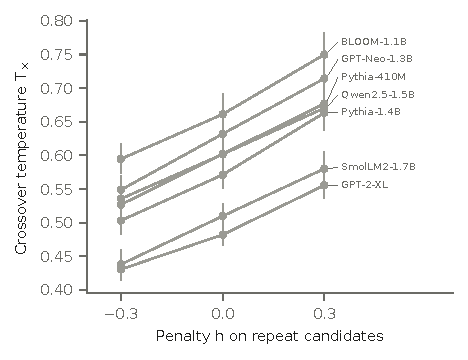
\includegraphics[width=\linewidth]{figures/figS1}
\caption{\textbf{Crossover temperature against the penalty.} $T_{\times}$ at $h$ = −0.3, 0 and +0.3 for the seven smaller models, from runs on the 40 design articles. Bars, 95\% bootstrap intervals over articles.}
\label{figS1}
\end{figure}

\begin{figure}
\renewcommand{\thefigure}{S2}
\centering
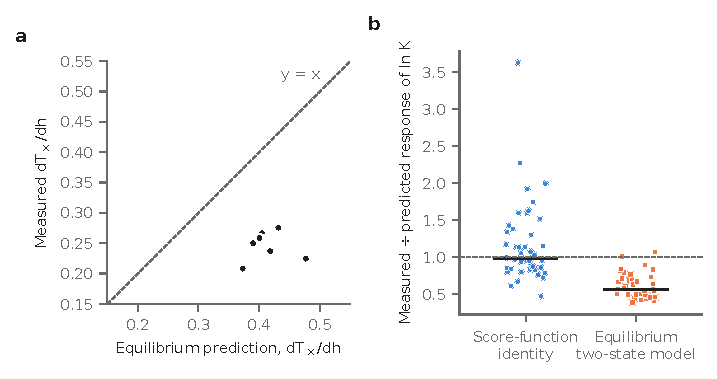
\includegraphics[width=\linewidth]{figures/figS2}
\caption{\textbf{Comparison with the equilibrium two-state model on the 40 design articles.} Panel a was preregistered; panel $b$ is a record without a decision rule. (a), Measured shift of $T_{\times}$ per unit $h$ against the equilibrium prediction $T_{\times}$ $\Delta c$/$\Delta E$. (b), Measured response of $\ln K$ to $h$ divided by the prediction of the exact derivative (left) and of the equilibrium two-state model (right), one point per model and temperature (7 × 7). Bars, medians. Computed per temperature and on these articles, the equilibrium median is 0.56, against $\rho_{\mathrm{eq}}$ = 0.69 summed over temperatures on the replication articles. The points within a model are not independent.}
\label{figS2}
\end{figure}

\subsection*{F1. Labeling checks}
\addcontentsline{toc}{subsection}{F1. Labeling checks}

All analyses in this subsection were exploratory. They used the unpenalized and penalized runs of the replication (seven smaller models) and of the test on the two larger models, 120 articles each. Their definitions and decision rules were fixed in a dated document before they were run. We also summed, over the usable temperatures of the unpenalized runs, the rate of choosing a repeat candidate in each state. In the repetitive and the ordinary state it was Pythia-410M 94\% and 20\%, Pythia-1.4B 94\% and 20\%, GPT-Neo-1.3B 94\% and 19\%, SmolLM2-1.7B 92\% and 21\%, Qwen2.5-1.5B 94\% and 17\%, GPT-2-XL 93\% and 19\%, BLOOM-1.1B 93\% and 17\%, Qwen2.5-7B 94\% and 16\%, Mistral-7B-v0.3 94\% and 20\%. These rates are a description computed after the tests.

\textbf{Switching near the crossover temperature.} For each model we took the test temperature closest to its unpenalized \(T_{\times}\) on the test grid. At that temperature each model had 480 unpenalized continuations, four per article. Between 74\% and 89\% of them switched state at least once (Table F1). Between 11\% and 26\% stayed in the ordinary state throughout. One continuation of Pythia-1.4B, and none of any other model, stayed repetitive throughout.

\textbf{Distribution of the windowed repeat fraction.} The windowed fraction \(k/32\) takes 33 values. We grouped them into a low side {[}0, 0.25), a middle {[}0.25, 0.75{]} and a high side (0.75, 1{]}. Before computing, we had called a model bimodal if the mean fraction of windows per bin in the middle was below one fifth of the smaller side. This had to hold both for all continuations and for the switching ones alone. No model met this criterion. Per bin, the middle held 0.008--0.014 of the windows, the low side 0.067--0.087 and the high side 0.021--0.033. Among switching continuations, the middle was 0.30--0.49 of the smaller side. The high side is small because continuations start in the ordinary state, and most of its mass lies in the bin at exactly one. The shape described in Sec. IV A is therefore present, but it does not meet the bimodality criterion fixed in advance.

\begin{table}[htbp]
\centering
\small
\setlength{\tabcolsep}{6pt}
\renewcommand{\thetable}{F1}
\caption{\textbf{Continuations near the crossover temperature.} \(T\): temperature of the test grid closest to \(T_{\times}\) estimated from the unpenalized runs of the same test. Switched: share of the 480 unpenalized continuations that switched state at least once. Ordinary: share that stayed ordinary throughout. Low, middle, high: mean fraction of windows per bin of the windowed repeat fraction, over all continuations. Middle/side: the middle per bin over the smaller side, switching continuations only; the bimodality criterion was a value below 0.2. \(T\) is chosen with \(T_{\times}\) from the straight-line fit; with the interpolated crossing of Appendix F6 it would be 0.57 instead of 0.62 for Pythia-1.4B and 0.55 instead of 0.60 for Qwen2.5-7B, and the same for the other seven models.}
\label{tabF1}
\begin{tabular}{@{}llllllll@{}}
\toprule
Model & \(T\) & Switched (\%) & Ordinary (\%) & Low & Middle & High & Middle/side \\
\midrule
Pythia-410M & 0.60 & 89 & 11 & 0.067 & 0.012 & 0.033 & 0.33 \\
Pythia-1.4B & 0.62 & 75 & 25 & 0.083 & 0.010 & 0.021 & 0.44 \\
GPT-Neo-1.3B & 0.63 & 83 & 17 & 0.074 & 0.011 & 0.027 & 0.39 \\
SmolLM2-1.7B & 0.51 & 88 & 12 & 0.069 & 0.014 & 0.027 & 0.49 \\
Qwen2.5-1.5B & 0.60 & 85 & 15 & 0.076 & 0.0093 & 0.030 & 0.30 \\
GPT-2-XL & 0.53 & 88 & 12 & 0.075 & 0.012 & 0.024 & 0.49 \\
BLOOM-1.1B & 0.66 & 80 & 20 & 0.077 & 0.011 & 0.025 & 0.41 \\
Qwen2.5-7B & 0.60 & 74 & 26 & 0.087 & 0.0075 & 0.022 & 0.31 \\
Mistral-7B-v0.3 & 0.49 & 81 & 19 & 0.080 & 0.010 & 0.024 & 0.39 \\
\bottomrule
\end{tabular}
\end{table}


\textbf{Eight other labelings.} We repeated the replication's test with windows of 16, 32 and 64 tokens and with entry and exit thresholds of (1/2, 1/4), (0.6, 0.3) and (0.4, 0.2). For each labeling we recomputed the states, the four counts, \(g\) and the usable temperatures, and kept \(h^*\) unchanged. The median ratio of the seven smaller models stayed within 0.8--1.25 under all eight other labelings, with points from 0.96 to 1.08 (Table F2). Longer windows gave slightly smaller ratios. For the smaller models the usable temperatures were the same under every labeling. For the two larger models the mean ratio under the eight other labelings was 0.87--0.95, against 0.96 under the original labeling, and with 64-token windows its interval reached below 0.8. Table F2 also lists \(\rho_{\mathrm{eq}}\) under each labeling, discussed in F7.

\begin{table}[htbp]
\centering
\small
\setlength{\tabcolsep}{6pt}
\renewcommand{\thetable}{F2}
\caption{\textbf{Replication ratio and \(\rho_{\mathrm{eq}}\) under nine labelings.} Window: length of the window for the repeat fraction, in tokens. Thresholds: windowed fraction at which a step enters and leaves the repetitive state. ρ: realized change in \(\ln K\) over the first-order prediction, median over the seven smaller models and mean over the two larger ones. \(\rho_{\mathrm{eq}}\): the same change over the equilibrium prediction with \(U\) = \(-\log p\), median over all nine models (F7). The first row is the labeling of the main text. Its point estimates equal those of the main text; its intervals for ρ differ slightly from Table I because this analysis used a different bootstrap seed, whereas \(\rho_{\mathrm{eq}}\) comes from the same analysis as Appendix H.}
\label{tabF2}
\begin{tabular}{@{}lllll@{}}
\toprule
Window & Thresholds & ρ, seven smaller & ρ, two larger & \(\rho_{\mathrm{eq}}\), nine models \\
\midrule
32 & (1/2, 1/4) & 1.04 (0.99--1.14) & 0.96 (0.85--1.13) & 0.69 (0.64--0.72) \\
16 & (1/2, 1/4) & 1.07 (1.01--1.16) & 0.92 (0.83--1.04) & 0.70 (0.65--0.74) \\
16 & (0.6, 0.3) & 1.07 (1.02--1.17) & 0.92 (0.83--1.06) & 0.74 (0.69--0.77) \\
16 & (0.4, 0.2) & 1.08 (1.01--1.16) & 0.92 (0.83--1.04) & 0.68 (0.64--0.72) \\
32 & (0.6, 0.3) & 1.05 (0.97--1.14) & 0.95 (0.84--1.12) & 0.71 (0.65--0.75) \\
32 & (0.4, 0.2) & 1.05 (0.98--1.14) & 0.93 (0.83--1.09) & 0.68 (0.63--0.71) \\
64 & (1/2, 1/4) & 0.97 (0.90--1.12) & 0.87 (0.75--1.07) & 0.66 (0.61--0.71) \\
64 & (0.6, 0.3) & 0.99 (0.89--1.10) & 0.92 (0.76--1.20) & 0.68 (0.61--0.73) \\
64 & (0.4, 0.2) & 0.96 (0.88--1.08) & 0.87 (0.75--1.07) & 0.63 (0.59--0.68) \\
\bottomrule
\end{tabular}
\end{table}


\subsection*{F2. Drift along the text and persistence of repetitive stretches}
\addcontentsline{toc}{subsection}{F2. Drift along the text and persistence of repetitive stretches}

Both analyses here were exploratory. They used the same runs and the same temperatures as F1.

\textbf{Drift.} We split the labeled pairs of steps into two halves by the first step of the pair, steps 16--255 and 256--495. At the temperature nearest \(T_{\times}\), \(\ln K\) lay between −1.54 and −0.64 in the first half and between 0.06 and 0.81 in the second (Table F3). The difference was between 1.3 and 2.1 in every model. The balance thus moves toward repetition along a text, and \(K\) is an average over positions. Because a window spans 32 steps, steps near the boundary also see marks from the other half.

\textbf{Persistence.} For each repetitive stretch whose entry was observed, we counted the steps \(d\) since entry and whether the state was left at the next step. Stretches still running at the end of the text were censored. We compared the exit hazard for \(d\ge 97\) with that for \(49\le d\le 96\). Shorter dwell times were excluded because the 32-token window and the hysteresis delay exits: an exit needs the windowed fraction to fall from 1/2 to below 1/4, which takes at least nine steps, and we placed the cut-off well above this. A synthetic Markov chain passed through the same marks and windows gives a ratio of about 0.99 for these two bins. A model was used only if each bin had at least ten exits.

The ratio of the hazard for long stretches to that for short ones had a median of 0.28 (0.23--0.34) over the nine models. It lay between 0.19 and 0.36 for each model, and every model's interval lay below 0.8 (Table F3). Each model had 62--139 exits in the shorter bin and 33--66 in the longer one. The same ratio for entering the repetitive state, after long and short ordinary stretches, was 0.77 (0.67--0.94).

This check does not separate three explanations. Stretches may become more stable as they last. Texts may differ in how easily they leave repetition, so that hard-to-leave texts fill the long bin. Position may also matter: the mean position of the steps at risk was 302--336 in the shorter bin and 363--386 in the longer one, where \(K\) is larger. Under any of these, the labeled states do not behave, at least as they stand, like a two-state Markov chain with fixed rates. This is why Sec. II treats \(K\) as a summary of switching statistics.

\begin{table}[htbp]
\centering
\small
\setlength{\tabcolsep}{6pt}
\renewcommand{\thetable}{F3}
\caption{\textbf{Drift and persistence near the crossover temperature.} \(T\): as in Table F1. \(\ln K\) in the first and second halves of the labeled steps. Exit ratio: exit hazard after 97 or more steps in the repetitive state over that after 49--96 steps. Entry ratio: the same for entering the repetitive state after long and short ordinary stretches.}
\label{tabF3}
\begin{tabular}{@{}llllll@{}}
\toprule
Model & \(T\) & \(\ln K\), first half & \(\ln K\), second half & Exit ratio & Entry ratio \\
\midrule
Pythia-410M & 0.60 & −0.64 & 0.73 & 0.19 (0.13--0.26) & 1.04 \\
Pythia-1.4B & 0.62 & −1.25 & 0.06 & 0.27 (0.17--0.41) & 0.60 \\
GPT-Neo-1.3B & 0.63 & −0.82 & 0.49 & 0.30 (0.21--0.43) & 0.78 \\
SmolLM2-1.7B & 0.51 & −0.74 & 0.63 & 0.36 (0.25--0.52) & 0.77 \\
Qwen2.5-1.5B & 0.60 & −1.00 & 0.81 & 0.33 (0.22--0.47) & 0.76 \\
GPT-2-XL & 0.53 & −1.09 & 0.33 & 0.23 (0.16--0.34) & 0.66 \\
BLOOM-1.1B & 0.66 & −0.96 & 0.48 & 0.34 (0.23--0.49) & 0.91 \\
Qwen2.5-7B & 0.60 & −1.54 & 0.55 & 0.28 (0.16--0.48) & 1.23 \\
Mistral-7B-v0.3 & 0.49 & −1.34 & 0.42 & 0.23 (0.15--0.35) & 0.74 \\
Median of nine & & & & 0.28 (0.23--0.34) & 0.77 (0.67--0.94) \\
\bottomrule
\end{tabular}
\end{table}


\subsection*{F3. First prospective test}
\addcontentsline{toc}{subsection}{F3. First prospective test}

This test was preregistered. It used the 40 design articles from which \(h^*\) had been computed, with arms at \(h^*\) and 2\(h^*\) for the seven smaller models. The decision rule was the one of Appendix C. Both arms were undecided: the median ratio was 1.17 (0.95--1.30) at \(h^*\) and 1.10 (0.97--1.30) at 2\(h^*\). The upper ends, 1.298 and 1.299, lay just above 1.25. For the median over models, doubling the penalty barely changed the ratio. Per model it rose at 2\(h^*\) for GPT-Neo-1.3B and GPT-2-XL (below), so linearity up to 2\(h^*\) holds for the median, not for every model. Per-model intervals were wide (Table F4). The difference between the medians at 2\(h^*\) and at \(h^*\) was −0.07 (−0.12 to 0.14); per model it excluded zero only for GPT-Neo-1.3B, +0.14 (0.04--0.24), and GPT-2-XL, +0.15 (0.005--0.47) (exploratory, record). \textbf{Second-order term.} The same score gives the second derivative from unpenalized samples, ∂²E{[}\(Y\){]}/∂h² = Cov(Y, S² − V)/T² with S = \(N\) − \(Q\) and V = \(\Sigma_{t}\) \(q_{t}\)(1 − \(q_{t}\)), and hence a second-order prediction \(h\) \(g\) + (h²/2) g₂. In an exploratory analysis made after these data had been seen, without a decision rule, this estimate was too noisy to use. Per model g₂/\(g\) ranged from −1.0 to +4.8, changed sign between the first test and the replication for some models, and in bootstrap resamples of five replication models its interval spanned roughly −2.5 to +3. Adding the second-order term moved the median ratio of the replication from 1.04 to 0.91 and that of the first test at \(h^*\) from 1.17 to 1.03, but at 2\(h^*\) from 1.10 to 1.65, away from one. An exactly solvable Markov model of copying, fitted earlier to two other language models, gave g₂/\(g\) of −0.06 to −0.13, which would raise the first-order ratio by a few percent at these penalties; this is a candidate explanation for ratios slightly above one, not a test.

This test was generated independently of the design runs: for the two models that shared six temperatures with them, no unpenalized continuation of the test repeated a design continuation token for token. We then committed, before any of its data existed, to the replication on 120 new articles reported in Sec. IV B.

\begin{table}[htbp]
\centering
\small
\setlength{\tabcolsep}{6pt}
\renewcommand{\thetable}{F4}
\caption{\textbf{First prospective test, 40 design articles.} \(h^*\): additive penalty used for generation, before division by temperature. Ratio: realized change in \(\ln K\) over the first-order prediction, summed over the usable temperatures, with a 95\% interval.}
\label{tabF4}
\begin{tabular}{@{}llll@{}}
\toprule
Model & \(h^*\) & Ratio at \(h^*\) & Ratio at 2\(h^*\) \\
\midrule
Pythia-410M & −0.40 & 1.18 (0.92--1.62) & 1.21 (0.96--1.65) \\
Pythia-1.4B & −0.50 & 0.75 (0.62--0.95) & 0.79 (0.66--1.00) \\
GPT-Neo-1.3B & −0.39 & 0.88 (0.66--1.22) & 1.01 (0.81--1.33) \\
SmolLM2-1.7B & −0.53 & 1.20 (0.96--1.62) & 1.09 (0.89--1.46) \\
Qwen2.5-1.5B & −0.47 & 1.07 (0.82--1.55) & 1.10 (0.88--1.55) \\
GPT-2-XL & −0.79 & 1.17 (0.95--1.54) & 1.32 (1.00--2.00) \\
BLOOM-1.1B & −0.37 & 1.25 (0.90--1.98) & 1.22 (0.88--1.93) \\
Median & & 1.17 (0.95--1.30) & 1.10 (0.97--1.30) \\
\bottomrule
\end{tabular}
\end{table}


\subsection*{F4. Prediction from the design data alone}
\addcontentsline{toc}{subsection}{F4. Prediction from the design data alone}

This analysis was exploratory. In the prospective tests only \(h^*\) was fixed in advance, and the predicted change \(h^*\) \(g\)(\(T\)) used \(g\) from the unpenalized arm of the same test. Here we used instead the prediction made at design time, \(h\bar{g}\) at every usable temperature. Here ḡ is the temperature-averaged \(g\) from the unpenalized design runs (Appendix C), and \(h\) is the rounded \(h^*\) used for generation. The ratio is \(\rho_{\mathrm{out}}\) = \(\Sigma_{u}\) Δ(\(T_{u}\))/(\(n_u h\bar{g}\)), with \(n_{u}\) the number of usable temperatures. Its intervals resample the 40 design articles, throug\(h\bar{g}\), and the 120 test articles separately, with 10,000 resamples; this rule was fixed before the analysis was run.

For the seven smaller models the median \(\rho_{\mathrm{out}}\) was 1.05 (0.93--1.20), inside 0.8--1.25 (Table F5). For the two larger models the mean was 1.07 (0.91--1.35), which left the test undecided. Wit\(h\bar{g}\) held fixed, the intervals would have been 0.99--1.11 and 1.01--1.14. The ratio \(\rho_{\mathrm{out}}\)/ρ equals the mean of \(g\)(\(T\)) over the usable temperatures divided by ḡ. It was 0.82--1.20 for the smaller models and 1.35 and 0.92 for the larger ones. A single design-time constant thus predicted the median change on new articles about as well as the test's own \(g\)(\(T\)) did. Individual models departed more, and only for GPT-2-XL, 1.29 (1.05--1.67), did the interval exclude one.

\textbf{Own or shared derivative.} The median rule does not require each model's own derivative. With each model's ḡ replaced by the mean ḡ of the other six smaller models, the median ratio was 1.09 (0.99--1.21), also inside the range. We measured the accuracy of a prediction by the median over the seven models of \textbar ln ρ\textbar. It was 0.062 with the model's own ḡ and 0.107 with the shared one, and their difference, 0.04 (−0.10 to 0.11), did not exclude zero when both sets of articles were resampled. For reference, the test's own \(g\) gave 0.057, and the slope measured on the design runs at \(h\) = ±0.3 gave 0.029, with a median ratio of 1.02 (0.95--1.09). Over resamples of the design articles the standard deviation of ḡ was 0.21--0.32 per unit of \(h\), and that of the measured slope 0.11--0.13, but the slope needs two penalized arms instead of one unpenalized arm.

\textbf{Fraction of repeats.} We also predicted the change in the fraction of the 512 steps marked as repeats, with the prediction \(h^*\) Cov(O, \(N\) − Q)/\(T\) for this fraction O in place of the one for \(\ln K\). Over the usable temperatures of the replication, the realized change over the predicted change had a median of 1.06 (1.00--1.15) for the smaller models and a mean of 0.91 (0.84--1.01) for the larger ones, both inside the range. For the fraction in the last 64 steps alone, the median for the smaller models was 1.23 (1.11--1.38), with its upper end above the range. The range was set for \(\ln K\), and this fraction uses the same repeat marks as the states, so it is not an independent check of \(s_{\mathrm{pen}}\).

\begin{table}[htbp]
\centering
\small
\setlength{\tabcolsep}{6pt}
\renewcommand{\thetable}{F5}
\caption{\textbf{Ratio to the design-time prediction.} ḡ: temperature-averaged ∂\(\ln K\)/∂\(h\) from the unpenalized design runs, per unit of \(h\). \(\rho_{\mathrm{out}}\): realized change in \(\ln K\) over \(h\bar{g}\), summed over the usable temperatures, with a 95\% interval that resamples the design and the test articles. ρ: the ratio of the prospective test (Table I).}
\label{tabF5}
\begin{tabular}{@{}lllll@{}}
\toprule
Model & ḡ & \(\rho_{\mathrm{out}}\) & ρ & \(\rho_{\mathrm{out}}\)/ρ \\
\midrule
Pythia-410M & 2.81 & 0.96 (0.80--1.20) & 1.12 & 0.86 \\
Pythia-1.4B & 2.44 & 1.06 (0.86--1.41) & 1.03 & 1.03 \\
GPT-Neo-1.3B & 2.52 & 1.05 (0.89--1.28) & 1.03 & 1.02 \\
SmolLM2-1.7B & 2.57 & 1.13 (0.92--1.41) & 1.18 & 0.95 \\
Qwen2.5-1.5B & 1.86 & 1.02 (0.75--1.54) & 0.94 & 1.07 \\
GPT-2-XL & 2.07 & 1.29 (1.05--1.67) & 1.08 & 1.20 \\
BLOOM-1.1B & 2.50 & 0.86 (0.68--1.15) & 1.04 & 0.82 \\
Median (first seven) & & 1.05 (0.93--1.20) & 1.04 & \\
Qwen2.5-7B & 1.30 & 1.19 (0.90--1.73) & 0.88 & 1.35 \\
Mistral-7B-v0.3 & 2.76 & 0.96 (0.76--1.24) & 1.04 & 0.92 \\
Mean (last two) & & 1.07 (0.91--1.35) & 0.96 & \\
\bottomrule
\end{tabular}
\end{table}


\subsection*{F5. Multiplicative penalty and instruction-tuned models}
\addcontentsline{toc}{subsection}{F5. Multiplicative penalty and instruction-tuned models}

All tests in this subsection were preregistered.

\textbf{Multiplicative penalty.} We used the definition of the widely used implementation in the Hugging Face transformers library. Before temperature scaling, the logit \(z\) of every token that has appeared earlier, including in the prompt, becomes \(z/\theta\) if \(z>0\) and \(z\theta\) otherwise. With λ = \(\ln \theta\), the derivative of a logit with respect to λ at λ = 0 is \(-|z|\) for seen tokens and zero otherwise. The identity then gives ∂\(\ln K\)/∂λ from unpenalized samples. We rescored the unpenalized samples of the earlier experiments without generating new text. We then predicted the \(\theta^*\) that lowers \(T_{\times}\) by 0.10, and fixed these predictions before sampling with \(\theta^*\). The control arm and the decision rule were those of the preregistered replication: 120 articles, the ratio of realized to predicted change in \(\ln K\), and the bootstrap interval of the median within 0.8--1.25.

\begin{table}[htbp]
\centering
\small
\setlength{\tabcolsep}{6pt}
\renewcommand{\thetable}{F6}
\caption{\textbf{Multiplicative penalty at the predicted divisor \(\theta^*\).} Ratio: realized change in \(\ln K\) over the first-order prediction, summed over the usable temperatures, with a 95\% interval over articles.}
\label{tabF6}
\begin{tabular}{@{}llll@{}}
\toprule
Model & \(\theta^*\) & Ratio & 95\% interval \\
\midrule
Pythia-410M & 1.021 & 0.99 & 0.85--1.20 \\
Pythia-1.4B & 1.027 & 1.12 & 0.94--1.39 \\
GPT-Neo-1.3B & 1.508 & 1.32 & 0.87--2.71 \\
SmolLM2-1.7B & 1.039 & 1.02 & 0.81--1.36 \\
Qwen2.5-1.5B & 1.022 & 0.94 & 0.79--1.18 \\
GPT-2-XL & 1.054 & 1.01 & 0.82--1.28 \\
BLOOM-1.1B & 1.019 & 0.91 & 0.76--1.12 \\
Median & & 1.01 & 0.92--1.14 \\
\bottomrule
\end{tabular}
\end{table}


The predicted divisors were 1.02--1.05 for six models and 1.51 for GPT-Neo-1.3B. For GPT-Neo-1.3B, the averaged response \(\bar{g}_{\lambda}\) of \(\ln K\) to λ = \(\ln \theta\) was 13--22 times smaller in magnitude than for the other models. The divisor acts on raw logits, so its effect depends on their scale in each model. The divisors of 1.1--1.3 common in practice correspond, for these six models, to 1.8 to 14 times the predicted ln \(\theta^*\); CTRL suggests about 1.2 \cite{1909.05858}.

\textbf{Stronger divisors.} In a further preregistered test, the divisor was set to \(\theta_k=e^{k\lambda^*}\), rounded to four decimals, with \(\lambda^*\) the predicted value of \(\ln \theta\) and \(k=2\), 4 and 8. It used the same 120 articles and temperatures, with the replication's unpenalized arm as control. Divisors above 3 were not run. GPT-Neo-1.3B was therefore tested at \(k=2\) only, and every decision used the other six models.

\begin{table}[htbp]
\centering
\small
\setlength{\tabcolsep}{6pt}
\renewcommand{\thetable}{F7}
\caption{\textbf{Stronger multiplicative penalties, six models.} k: multiple of the predicted \(\lambda^*\). θ: divisors used for the six models. Ratio: median over the six models (five at \(k=8\), where Pythia-410M dropped out), with a 95\% interval. The \(k=1\) row is Table F6 without GPT-Neo-1.3B, so its median differs from the median over seven models.}
\label{tabF7}
\begin{tabular}{@{}lllll@{}}
\toprule
k & θ (six models) & Median ratio & 95\% interval & Decision \\
\midrule
1 & 1.02--1.05 & 1.00 & 0.91--1.11 & (replication, for reference) \\
2 & 1.04--1.11 & 1.00 & 0.90--1.12 & within the range \\
4 & 1.08--1.24 & 0.86 & 0.77--0.99 & undecided \\
8 & 1.17--1.53 & 0.52 & 0.46--0.67 & below the range \\
\bottomrule
\end{tabular}
\end{table}


At \(k=8\) the penalty suppressed repetition so strongly that Pythia-410M kept only one usable temperature and dropped out. Three other models kept two or three. Models differed in how fast the ratio fell. SmolLM2-1.7B reached 0.24 at \(k=8\), whereas both Pythia models stayed near 1 up to \(k=4\). GPT-Neo-1.3B at \(k=2\) (θ = 2.27) gave 1.64 (1.11--3.59). Its point estimate was the only one well above one, but its interval reached into the range, so the rule did not call it larger than predicted.

\textbf{Instruction-tuned models.} Prompts were wrapped in each model's chat template. The user turn was ``Continue this news article:'' followed by the first 64 tokens of the article. \(T_{\times}\) was located from 15 temperatures between 0.20 and 0.90, as for the larger models. For Qwen2.5-1.5B-Instruct the unpenalized \(T_{\times}\) was 0.65, and the predicted additive penalty was \(h^*\) = −0.33. The ratio was 1.36 (0.81--2.40), which neither confirms nor rejects the prediction. For SmolLM2-1.7B-Instruct the provisional \(T_{\times}\) was 0.16. This lay outside the range in which our procedure makes a prediction (0.3--0.8), so no test was run.

\subsection*{F6. Shift of the crossover temperature}
\addcontentsline{toc}{subsection}{F6. Shift of the crossover temperature}

Three analyses bear on where \(T_{\times}\) ended up. All three were defined after the main test had been analyzed, and we report them as exploratory. For the straight-line comparison, the question and decision rule were fixed in a dated document before \(T_{\times}\) was computed for these runs; for the interpolated crossing, a rule was fixed before it was computed, and the quadratic fit was a record.

\textbf{Straight-line fit.} In each arm we fitted \(\ln K=a+b/T\) over the usable temperatures of the test grid and took \(T_\times=-b/a\). The shift divided by the intended −0.10 had a median of 1.32 (1.18--1.50) for the smaller models, which was undecided. For the larger models the mean was 2.17 (1.90--2.54), larger than intended. For GPT-2-XL and the two larger models, the unpenalized \(T_{\times}\) lay outside the test grid and was extrapolated.

\textbf{Interpolated crossing.} Since \(\ln K\) curves in 1/\(T\), we also located each crossing without a fit. We sorted the usable temperatures of each arm by 1/\(T\) and took the adjacent pair between which \(\ln K\) rises through zero. We then interpolated linearly in 1/\(T\). If there were several such pairs, we took the one nearest a guide fixed beforehand: the design \(T_{\times}\) for the unpenalized arm and \(T^*\) for the penalized arm. Every arm of every model crossed zero inside its grid, so no extrapolation was needed.

With the interpolated crossings, the ratio became smaller for every one of the nine models (Table F8). The median over the smaller models was 0.87 (0.80--1.03), inside 0.8--1.25. The mean over the larger models was 1.33 (1.14--1.53). The roots of a quadratic fit gave a median of 0.95 (0.86--1.07). The unpenalized crossing lay 0.002--0.024 above the design \(T_{\times}\) in seven models and about 0.01 below it in two. Thus it sat near the upper edge of the test grid, where a straight line fitted over the whole grid is least accurate. The penalized crossing lay within 0.04 of \(T^*\) for seven models, BLOOM-1.1B at exactly +0.040. It lay 0.057 below \(T^*\) for SmolLM2-1.7B and 0.117 below for GPT-2-XL. GPT-2-XL and SmolLM2-1.7B still moved by more than intended, with intervals above 1.25, and BLOOM-1.1B moved by less, with an interval below 0.8. The mean over the larger models stayed above 1.25 in its point estimate. No per-model interval of the interpolated ratio lay inside 0.8--1.25.

\textbf{Why the shift missed in some models.} This check was made after the tests and is a record. The derivative of Sec. III A also predicts the slope of \(T_{\times}\) in \(h\), \(g\)(\(T_{\times}\)) T\_ײ/\(b\) at the crossover. On the design runs this predicted slope agreed with the measured slope of Fig. S1 to within a quarter in every smaller model; for GPT-2-XL they were 0.206 and 0.208. Multiplying the measured slope by \(h^*\) gives the shift that the design data implied: 0.99, 1.33, 1.07, 1.25, 1.05, 1.64 and 0.97 times the intended 0.10, in the order of Table I. \(h^*\) had instead been set wit\(h\bar{g}\), the average of \(g\) over 0.40--0.70, and with the straight-line \(T_{\times}\). \(g\) at the crossover over ḡ was 1.07, 1.13, 1.17, 1.20, 1.10, 1.28 and 0.83 in the same order. The largest overshoot, for GPT-2-XL, was thus visible in the design data and follows from using a temperature-averaged derivative where \(g\) changes with temperature; BLOOM-1.1B, the one model with \(g\)(\(T_{\times}\)) below ḡ, undershot.

\begin{table}[htbp]
\centering
\small
\setlength{\tabcolsep}{6pt}
\renewcommand{\thetable}{F8}
\caption{\textbf{Shift of the crossover temperature.} \(T^*\): design temperature. Offsets: interpolated unpenalized crossing minus the design \(T_{\times}\), and interpolated penalized crossing minus \(T^*\). Ratios: shift of \(T_{\times}\) divided by the intended −0.10, from a straight-line fit and from interpolation, with a 95\% interval for the latter.}
\label{tabF8}
\begin{tabular}{@{}llllll@{}}
\toprule
Model & \(T^*\) & Unpenalized offset & Penalized offset & Straight-line ratio & Interpolated ratio \\
\midrule
Pythia-410M & 0.50 & +0.006 & +0.025 & 1.13 & 0.81 (0.71--0.90) \\
Pythia-1.4B & 0.47 & +0.007 & −0.010 & 1.55 & 1.16 (1.02--1.28) \\
GPT-Neo-1.3B & 0.53 & −0.009 & +0.006 & 1.02 & 0.85 (0.74--0.96) \\
SmolLM2-1.7B & 0.41 & +0.002 & −0.057 & 2.05 & 1.60 (1.43--1.81) \\
Qwen2.5-1.5B & 0.50 & +0.004 & +0.016 & 1.32 & 0.87 (0.70--1.02) \\
GPT-2-XL & 0.38 & +0.024 & −0.117 & 3.10 & 2.41 (2.19--2.79) \\
BLOOM-1.1B & 0.56 & −0.010 & +0.040 & 0.79 & 0.51 (0.39--0.63) \\
Median (first seven) & & & & 1.32 (1.18--1.50) & 0.87 (0.80--1.03) \\
Qwen2.5-7B & 0.45 & +0.014 & −0.039 & 2.25 & 1.53 (1.23--1.86) \\
Mistral-7B-v0.3 & 0.34 & +0.024 & +0.010 & 2.10 & 1.14 (0.91--1.35) \\
Mean (last two) & & & & 2.17 (1.90--2.54) & 1.33 (1.14--1.53) \\
\bottomrule
\end{tabular}
\end{table}


\textbf{Penalized \(\ln K\) at the design temperature.} The design line \(a+b/T+h\bar{g}\) crosses zero at \(T^*\) by construction. At the test temperature closest to \(T^*\), the center of each grid, we compared the penalized \(\ln K\) with this line. The deviation splits exactly into three parts. The first is the deviation of the unpenalized \(\ln K\) from \(a+b/T\). The second is \(h[g(T)-\bar{g}]\), the change of \(g\) with temperature. The third is Δ(\(T\)) − \(h\) \(g\)(\(T\)), the departure from the identity. We count each part as positive when it would lower \(T_{\times}\) further.

The median total deviation over the nine models was −0.05 (−0.17 to 0.12). At the design temperature the penalized \(\ln K\) was thus close to its target. The first two parts had medians of −0.02 (−0.15 to 0.10) and −0.03 (−0.24 to 0.12), and neither interval excluded zero. Per model, the total ranged from −0.48 for BLOOM-1.1B to 0.87 for GPT-2-XL. The first part combined two opposing pieces. In every model, the unpenalized \(\ln K\) at the grid center lay 0.16--0.34 above the straight line fitted on the same grid, so \(\ln K\) is concave in 1/\(T\). The line fitted on the test grid also lay below the design line there, by 0.08--0.70, in eight models; for BLOOM-1.1B it lay 0.09 above. The overshoot of \(T_{\times}\) therefore does not come from a misprediction of \(\ln K\) at \(T^*\).

\subsection*{F7. Records for the equilibrium two-state model}
\addcontentsline{toc}{subsection}{F7. Records for the equilibrium two-state model}

\textbf{Recorded factor \(r_{C}\) and \(\rho_{\mathrm{eq}}\).} Before each test we wrote into the prediction file a factor \(r_{C}\). It is the shift of \(T_{\times}\) that the equilibrium two-state model predicts at \(h^*\), divided by the intended 0.10. \(r_{C}\) was computed from the design data, as \textbar{}\(h^*\)\textbar{} \(T_{\times}\) \(\Delta c\)/(0.10 \(\Delta E\)). It was 1.5--2.9 for the smaller models and 3.4 and 1.7 for the larger ones (Table F9). No decision rule was attached to it. Table F9 sets it beside two later comparisons and beside \(\rho_{\mathrm{eq}}\).

The first comparison divides the realized shift of the straight-line \(T_{\times}\) by −0.10 \(r_{C}\), a ratio in \(T_{\times}\) throughout. It ranged from 0.53 to 1.26, with a median of 0.73 over nine models. \(\rho_{\mathrm{eq}}\) instead builds the equilibrium prediction at each temperature from the unpenalized arm of the same test, in \(\ln K\). It was computed after the tests and ranged from 0.52 to 0.98, with a median of 0.69 (0.64--0.72). Appendix H uses \(\rho_{\mathrm{eq}}\). Both measures agree that the two-state model overstated the response in most models. They differ most for Mistral-7B-v0.3, 1.26 against 0.96.

\begin{table}[htbp]
\centering
\small
\setlength{\tabcolsep}{6pt}
\renewcommand{\thetable}{F9}
\caption{\textbf{Equilibrium two-state model: recorded factor and later ratios.} \(r_{C}\): shift of \(T_{\times}\) predicted by the equilibrium two-state model at \(h^*\), over the intended 0.10, written before each test. ρ: test ratio (Table I). \(T_{\times}\) ratio: realized shift of the straight-line \(T_{\times}\) over −0.10 \(r_{C}\). \(\rho_{\mathrm{eq}}\): realized change in \(\ln K\) over the equilibrium prediction built at each temperature, with a 95\% interval.}
\label{tabF9}
\begin{tabular}{@{}lllll@{}}
\toprule
Model & \(r_{C}\) & ρ & \(T_{\times}\) ratio & \(\rho_{\mathrm{eq}}\) \\
\midrule
Pythia-410M & 1.54 & 1.12 & 0.73 & 0.69 (0.64--0.74) \\
Pythia-1.4B & 2.01 & 1.03 & 0.77 & 0.70 (0.64--0.77) \\
GPT-Neo-1.3B & 1.68 & 1.03 & 0.61 & 0.63 (0.58--0.69) \\
SmolLM2-1.7B & 2.21 & 1.18 & 0.93 & 0.85 (0.79--0.92) \\
Qwen2.5-1.5B & 2.24 & 0.94 & 0.59 & 0.55 (0.50--0.61) \\
GPT-2-XL & 2.93 & 1.08 & 1.06 & 0.98 (0.91--1.06) \\
BLOOM-1.1B & 1.50 & 1.04 & 0.53 & 0.52 (0.47--0.58) \\
Qwen2.5-7B & 3.36 & 0.88 & 0.67 & 0.58 (0.52--0.66) \\
Mistral-7B-v0.3 & 1.66 & 1.04 & 1.26 & 0.96 (0.84--1.09) \\
Median of nine & & & 0.73 & 0.69 (0.64--0.72) \\
\bottomrule
\end{tabular}
\end{table}


\textbf{Halves and labelings.} These analyses were exploratory. We recomputed the counts, \(\Delta c\), \(\Delta E\), \(b\) and \(g\) separately for the first and second halves of the labeled steps, as in F2, keeping σ over the whole text. The median \(\rho_{\mathrm{eq}}\) was 0.73 (0.67--0.80) in the first half and 0.59 (0.55--0.62) in the second. The upper end in the first half, 0.8003, just failed the rule fixed beforehand, an upper end below 0.8; we read this as a boundary case rather than a difference between the halves. The ratio of the first-order prediction stayed close to one in both halves, 1.10 (0.99--1.19) and 0.91 (0.82--1.04). Under the eight other labelings of F1, \(\rho_{\mathrm{eq}}\) ranged from 0.63 to 0.74 (Table F2). These checks do not show that the drift along the text plays no role.

\textbf{Per-temperature comparison on the design articles (Fig. S2).} These runs used the 40 design articles, seven temperatures from 0.40 to 0.70 and \(h\) = −0.3, 0 and +0.3, for the seven smaller models. One comparison was preregistered. We defined \(R\) as the measured slope \(dT_\times/dh\) divided by the equilibrium prediction \(T_{\times}\) \(\Delta c\)/\(\Delta E\). \(R\) would count as smaller than predicted if its interval lay below 0.8. This held for all seven models, with \(R\) between 0.47 and 0.66 and a median of 0.64 (Table F10; Fig. S2a).

The per-temperature comparison of Fig. S2b was a record, not a decision. At each temperature, the measured response of \(\ln K\) was (\(\ln K\)(+0.3) − \(\ln K\)(−0.3))/0.6. Divided by the first-order prediction from the \(h\) = 0 arm, it had a median of 0.98 over the 49 model--temperature pairs. Divided by the equilibrium prediction \(g_{C}\)(\(T\)) of Appendix H, it had a median of 0.56. The points within a model are not independent. The value 0.56 is lower than \(\rho_{\mathrm{eq}}\) = 0.69 on the replication. The two differ in articles and penalty strength, and \(\rho_{\mathrm{eq}}\) sums over temperatures instead of taking a median.

\begin{table}[htbp]
\centering
\small
\setlength{\tabcolsep}{6pt}
\renewcommand{\thetable}{F10}
\caption{\textbf{Design runs: shift of \(T_{\times}\) and per-temperature response.} \(T_{\times}\): unpenalized crossover temperature on the design grid. Slope: measured \(dT_\times/dh\). Prediction: equilibrium prediction \(T_{\times}\) \(\Delta c\)/\(\Delta E\). \(R\): slope over prediction, with a 95\% interval. Identity and equilibrium: median over the seven temperatures of the measured response of \(\ln K\) over each prediction.}
\label{tabF10}
\begin{tabular}{@{}lllllll@{}}
\toprule
Model & \(T_{\times}\) & Slope & Prediction & \(R\) & Identity & Equilibrium \\
\midrule
Pythia-410M & 0.60 & 0.25 & 0.39 & 0.64 (0.57--0.73) & 0.95 & 0.66 \\
Pythia-1.4B & 0.57 & 0.27 & 0.40 & 0.66 (0.59--0.74) & 1.15 & 0.60 \\
GPT-Neo-1.3B & 0.63 & 0.28 & 0.43 & 0.64 (0.56--0.74) & 0.98 & 0.58 \\
SmolLM2-1.7B & 0.51 & 0.24 & 0.42 & 0.57 (0.51--0.64) & 0.99 & 0.56 \\
Qwen2.5-1.5B & 0.60 & 0.22 & 0.48 & 0.47 (0.40--0.54) & 0.94 & 0.45 \\
GPT-2-XL & 0.48 & 0.21 & 0.37 & 0.56 (0.50--0.62) & 1.60 & 0.64 \\
BLOOM-1.1B & 0.66 & 0.26 & 0.40 & 0.65 (0.54--0.76) & 0.97 & 0.52 \\
All 49 pairs & & & & & 0.98 & 0.56 \\
\bottomrule
\end{tabular}
\end{table}


\subsection*{\texorpdfstring{F8. The fraction \(s_{\mathrm{pen}}\) against text length and covariance convention}{F8. The fraction s\_\{\textbackslash mathrm\{pen\}\} against text length and covariance convention}}
\addcontentsline{toc}{subsection}{F8. The fraction \(s_{\mathrm{pen}}\) against text length and covariance convention}

This analysis was exploratory. \(s_{\mathrm{pen}}\) is \(\Sigma_{u}\) \(g\)/\(\Sigma_{u}\) \(g_{N}\) over the usable temperatures of the unpenalized arms, as in Table II. The baseline uses covariances within articles and texts of 512 tokens (Appendix B). We changed one choice at a time. In the mixed convention, the numerator \(g\) used covariances pooled over all articles, as in the tests, and the denominator stayed within articles. For shorter texts we recomputed the repeat marks, states, counts, \(N\), \(Q\) and usable temperatures from the first \(L\)′ steps only. Before computing, we called \(s_{\mathrm{pen}}\) ``about 1\%'' if the interval of the median lay within 0.5--2\%.

The two conventions gave nearly the same median, 1.16\% (1.08--1.31) at baseline and 1.17\% (1.05--1.30) in the mixed convention (Table F11). This is expected, because \(N\) − \(Q\) has mean zero within each article. Pooling both numerator and denominator over articles gave 0.90\% (0.79--1.01). That is a different quantity, since differences between articles then enter the denominator. Shorter texts kept more: 1.38\% (1.25--1.51) for 384 tokens and 1.79\% (1.63--1.94) for 256 tokens. On temperatures \(u\)sable at both lengths, \(s_{\mathrm{pen}}\) at 256 tokens was 1.48 (1.37--1.60) times that at 512. All three medians that had a decision rule fell within 0.5--2\%. For the individual smaller models at 256 tokens, \(s_{\mathrm{pen}}\) ranged from 1.46\% to 2.05\%; for the two larger models it was 1.08\% and 1.30\%. The first 256 tokens also come from the part of a text where repetition has not yet developed, so length and position are confounded.

\textbf{Relaxation time.} Before computing τ (Table II) we fixed how to read \(s_{\mathrm{pen}}\) τ across the seven smaller models: a coefficient of variation below 0.3 would count as consistent with the reading that \(s_{\mathrm{pen}}\) is about one over the relaxation time, and one above 0.6 as inconsistent. It was 0.14, with \(s_{\mathrm{pen}}\) τ between 0.99 and 1.50. The rank correlation between \(s_{\mathrm{pen}}\) and 1/τ over the same models was only 0.11, so the reading fixes the size of \(s_{\mathrm{pen}}\), not its order across models. The coefficient of variation of \(s_{\mathrm{pen}}\) alone was 0.16 and that of τ 0.09, so the criterion would have been met even for unrelated values; it could not discriminate, and we do not use it as support.

\begin{table}[htbp]
\centering
\small
\setlength{\tabcolsep}{6pt}
\renewcommand{\thetable}{F11}
\caption{\textbf{Surviving fraction \(s_{\mathrm{pen}}\) (\%) under different conventions.} Baseline: covariances within articles, 512 tokens. Mixed: numerator pooled over articles. Pooled: numerator and denominator pooled over articles. \(L\)′: only the first \(L\)′ generated tokens. The median row gives medians over the seven smaller models, with 95\% intervals. Dashes mark values not computed.}
\label{tabF11}
\begin{tabular}{@{}llllll@{}}
\toprule
Model & Baseline & Mixed & Pooled & \(L\)′ = 384 & \(L\)′ = 256 \\
\midrule
Pythia-410M & 1.29 & 1.28 & 0.97 & 1.45 & 1.80 \\
Pythia-1.4B & 1.33 & 1.33 & 0.99 & 1.51 & 1.79 \\
GPT-Neo-1.3B & 1.46 & 1.40 & 1.13 & 1.73 & 2.05 \\
SmolLM2-1.7B & 1.07 & 1.07 & 0.83 & 1.38 & 1.90 \\
Qwen2.5-1.5B & 0.81 & 0.84 & 0.65 & 1.06 & 1.46 \\
GPT-2-XL & 1.13 & 1.05 & 0.77 & 1.30 & 1.67 \\
BLOOM-1.1B & 1.16 & 1.17 & 0.90 & 1.21 & 1.74 \\
Median (first seven) & 1.16 (1.08--1.31) & 1.17 (1.05--1.30) & 0.90 (0.79--1.01) & 1.38 (1.25--1.51) & 1.79 (1.63--1.94) \\
Qwen2.5-7B & 0.68 & 0.66 & --- & --- & 1.08 \\
Mistral-7B-v0.3 & 0.68 & 0.66 & --- & --- & 1.30 \\
\bottomrule
\end{tabular}
\end{table}


\subsection*{F9. Other genres}
\addcontentsline{toc}{subsection}{F9. Other genres}

This experiment was preregistered. It repeated the design runs of F7 on three other kinds of text, for four of the smaller models: Pythia-1.4B, SmolLM2-1.7B, Qwen2.5-1.5B and BLOOM-1.1B. The prompts were 40 arXiv papers from April and May 2025, 35 code files from December 2024 to June 2025, and 40 English novels from Project Gutenberg. Two questions were fixed in advance. The first asked whether \(T_{\times}\) rose with \(h\) beyond what the labeling alone produces. The second asked whether \(R\), defined as in F7, was smaller than predicted.

The first question compared the slope of \(T_{\times}\) in \(h\) with the apparent slope that the labeling itself produces under the penalty, measured on a synthetic process without switching (at most 0.02 per unit h), for two labelings. \(T_{\times}\) rose beyond it in 11 of the 12 model--genre pairs. For papers and novels, \(R\) lay between 0.42 and 0.65, as for news (Table F12). The decision was ``smaller than predicted'' for novels in four of four models and for papers in three of four. For BLOOM-1.1B on papers, \(R\) pointed below one, but its interval reached 0.82, just above the 0.8 of the rule. Its rise of \(T_{\times}\) also could not be separated from the effect of the labeling alone. Code could not be measured: in all four models the unpenalized \(T_{\times}\) lay between 1.2 and 1.7, far above the sampled range. Its intervals for \(R\) were therefore very wide, and the overall decision was undecided. In all 12 pairs the first-order prediction was closer to the measured response of \(\ln K\) than the equilibrium two-state model. These ratios have no intervals and were not part of the decision.

\begin{table}[htbp]
\centering
\small
\setlength{\tabcolsep}{6pt}
\renewcommand{\thetable}{F12}
\caption{\textbf{Other genres, design runs.} \(T_{\times}\): unpenalized crossover temperature; values above 0.7 are extrapolated. \(R\): measured \(dT_\times/dh\) over the equilibrium prediction, with a 95\% interval. Identity and equilibrium: measured response of \(\ln K\) over each prediction, summed over the seven temperatures. News: the same four models on the 40 design articles. The \(T_{\times}\) and \(R\) values are those of Table F10; the identity and equilibrium columns here are sums over temperatures, whereas Table F10 gives medians over temperatures.}
\label{tabF12}
\begin{tabular}{@{}llllll@{}}
\toprule
Genre & Model & \(T_{\times}\) & \(R\) & Identity & Equilibrium \\
\midrule
Papers & Pythia-1.4B & 0.67 & 0.42 (0.30--0.53) & 0.88 & 0.46 \\
Papers & SmolLM2-1.7B & 0.58 & 0.65 (0.53--0.79) & 1.09 & 0.61 \\
Papers & Qwen2.5-1.5B & 0.62 & 0.48 (0.38--0.62) & 1.08 & 0.48 \\
Papers & BLOOM-1.1B & 0.69 & 0.58 (0.44--0.82) & 0.71 & 0.46 \\
Novels & Pythia-1.4B & 0.64 & 0.42 (0.36--0.48) & 1.20 & 0.44 \\
Novels & SmolLM2-1.7B & 0.57 & 0.46 (0.40--0.53) & 1.15 & 0.45 \\
Novels & Qwen2.5-1.5B & 0.63 & 0.49 (0.42--0.60) & 0.84 & 0.47 \\
Novels & BLOOM-1.1B & 0.68 & 0.48 (0.39--0.59) & 0.80 & 0.46 \\
Code & Pythia-1.4B & 1.24 & 0.47 (0.11--1.48) & 0.76 & 0.28 \\
Code & SmolLM2-1.7B & 1.29 & 0.31 (−0.02--0.90) & 0.87 & 0.38 \\
Code & Qwen2.5-1.5B & 1.23 & 0.78 (0.19--3.62) & 1.05 & 0.33 \\
Code & BLOOM-1.1B & 1.74 & 0.66 (0.03--4.57) & 1.46 & 0.37 \\
News & Pythia-1.4B & 0.57 & 0.66 (0.59--0.74) & 1.05 & 0.59 \\
News & SmolLM2-1.7B & 0.51 & 0.57 (0.51--0.64) & 0.94 & 0.55 \\
News & Qwen2.5-1.5B & 0.60 & 0.47 (0.40--0.54) & 1.00 & 0.47 \\
News & BLOOM-1.1B & 0.66 & 0.65 (0.54--0.76) & 0.92 & 0.58 \\
\bottomrule
\end{tabular}
\end{table}


\subsection*{F10. Per-temperature agreement, the split between the rates, and the choice of temperatures}
\addcontentsline{toc}{subsection}{F10. Per-temperature agreement, the split between the rates, and the choice of temperatures}

These analyses were exploratory, with rules fixed in a dated document before they were run, and used the runs of the replication and of the test on the larger models.

First, the test sums the realized and predicted changes over temperatures, so errors at single temperatures could cancel. For each model we fitted a straight line to the ratio of realized to predicted change against temperature and took its change across the usable temperatures. The median over the smaller models was 0.01 (−0.446 to 0.161), just inside ±0.45, the width of the decision range, which a rule fixed beforehand read as no drift beyond that width. The lower end lies on the boundary, so this result does not exclude a drift of that size. For the two larger models the mean was −0.13 (−1.41 to 0.29), which did not decide. Single temperatures were imprecise: the half-width of the interval of the difference between realized and predicted change had a median of 39\% of the prediction. Of the 49 model--temperature pairs of the smaller models, 4 had an interval excluding zero, 8\% against the 5\% expected by chance, all four with the realized change below the predicted one, and of the 14 pairs of the larger models, 1.

Second, Fig. 3b compared the predicted share of the entry rate, as a point, with the interval of the measured share. Computing the difference within the same resamples includes the uncertainty of both. The median difference over the smaller models was −0.04 (−0.11 to −0.002), so the identity put slightly more of the response on the exit rate; for the larger models the mean was −0.03 (−0.11 to 0.05). The difference excluded zero for Pythia-1.4B and GPT-2-XL, against six models in the comparison with a point.

Third, a temperature was usable if both kinds of switch occurred at least ten times in both arms. We also tried four other rules: the unpenalized arm alone, at least five or at least twenty switches, and choosing again in every resample. None changed the set of temperatures for any model: every model used all seven temperatures of its grid, every temperature had at least twenty switches of each kind in both arms, and no resample changed the set. The choice of usable temperatures therefore did not affect the result, and the rule fixed beforehand recorded this question as undecided because no alternative rule could be tested.

\section{Truncated sampling}

Truncated samplers such as min-p \cite{2407.01082} and top-p \cite{1904.09751} select a set \(S_{t}\) of allowed tokens and renormalize within it. If no token lies on the boundary of \(S_{t}\) at \(h\) = 0, the set is fixed for small \(h\) and the score of Sec. III A holds with \(q_{t}\) replaced by the probability of the repeat candidates after renormalization within \(S_{t}\); for min-p with threshold r this is guaranteed at every step whose margin \(min_{v}\) \textbar{}\(z_{v}\)/\(T\) − \(max_{u}\) \(z_{u}\)/\(T\) − ln r\textbar{} exceeds \textbar{}\(h\)\textbar/\(T\). We checked this exactly in a toy model with five tokens and five steps, for both penalties and both truncations, but not with language models.

\section{The equilibrium two-state model}

\textbf{Definition.} Suppose each state were a Boltzmann ensemble of independent units of \(m\) steps, with energy difference \(m\Delta E\) per unit between the states. Here \(\Delta E\) is the difference in mean energy per step, ordinary minus repetitive. The van 't Hoff slope would then be \(b=\partial\ln K/\partial\beta=m\Delta E\). A penalty \(h\) per chosen candidate would shift the free-energy difference per unit by \(h\) \(m\Delta c\), where \(\Delta c\) is the rate of choosing a candidate in the repetitive state minus that in the ordinary state. Hence the equilibrium prediction is

\begin{equation}g_C(T)=\frac{b}{\Delta E}\,\frac{\Delta c_T}{T},\end{equation}

with \(b\), \(\Delta E\) and \(\Delta c_{T}\), the value of \(\Delta c\) at temperature \(T\), all measured without the penalty; \(\Delta E\) is averaged over the usable temperatures. The same form built from exponential tilting uses \(b_{\mathrm{tilt}}\) in place of \(b\); we write it \(g_{C}^{\mathrm{tilt}}\).

\textbf{Temperature.} Changing the temperature is also a step-wise change. With β = 1/\(T\) and energy \(U_{t}\) = \(-\log p_t\) at \(T\) = 1,

\begin{equation}\frac{\partial \log P_\beta(x)}{\partial\beta}=-\big(U-U_{\mathrm{comp}}\big),\qquad U=\sum_t U_t(x_t),\quad U_{\mathrm{comp}}=\sum_t E_t[U_t],\end{equation}

where \(E_{t}\) is the expectation under the step-\(t\) distribution at the current temperature. The van 't Hoff slope \(b\) = ∂ \(\ln K\)/∂β, the slope of \(\ln K\) against 1/\(T\), measures this step-wise response to temperature, which therefore also subtracts a compensator. Exponential tilting by \(\exp(-\varepsilon U)\), with a small tilt ε, does not. Because each step's expectation is subtracted, adding to \(U_{t}\) any constant that depends only on the history, for example replacing \(U_t\) by \(-z_t\), leaves this score unchanged. The corresponding fraction for temperature is \(s_{\mathrm{temp}}\) = \(b\)/\(b_{\mathrm{tilt}}\), where \(b_{\mathrm{tilt}}\) is the response of \(\ln K\) to exponential tilting by \(\exp(-\varepsilon U)\) at ε = 0. Over several temperatures we sum numerator and denominator with the weights of the equilibrium prediction \(g_{C}\) above: \(s_{\mathrm{temp}}=\sum_u g_C(T_u)/\sum_u g_C^{\mathrm{tilt}}(T_u)\). Here \(g_{C}^{\mathrm{tilt}}\) is \(g_{C}\) with \(b_{\mathrm{tilt}}\) in place of \(b\).

With \(s_{\mathrm{pen}}\) and \(s_{\mathrm{temp}}\), the ratio of the exact response to the equilibrium prediction factorizes as

\begin{equation}\frac{g}{g_C}=\frac{s_{\mathrm{pen}}}{s_{\mathrm{temp}}}\,\kappa,\qquad \kappa=\frac{g_N}{g_C^{\mathrm{tilt}}}.\end{equation}

The factorization is an identity, at each temperature and, with each factor a ratio of sums over the usable temperatures, for the sums as well; its content lies in the sizes of the factors. The prediction is right only if κ \(s_{\mathrm{pen}}\) = \(s_{\mathrm{temp}}\). κ compares the two tilted responses, where no step-wise normalization intervenes. κ ≈ 1 is what the two-state form predicts, but it would also follow if one slow mode dominated both responses. Because \(b\) is the slope of a straight-line fit over several temperatures whereas \(g\) is local, curvature of \(\ln K\) alone makes \(g\)/\(g_{C}\) depend on temperature.

\(\Delta E\) depends on the energy assigned to a step. We use \(U_{t}\) = \(-\log p_t\) at \(T\) = 1, the energy that makes each step exactly Boltzmann at \(T\) = 1. Adding to \(U_{t}\) a constant that depends on the history changes \(\Delta E\), \(b_{\mathrm{tilt}}\), κ and \(s_{\mathrm{temp}}\), and hence \(g_{C}\), but not \(g\), \(s_{\mathrm{pen}}\) or \(b\).

\textbf{Prediction of the shift of \(T_{\times}\) and of \(\ln K\).} Applying the implicit-function theorem to \(\ln K\) = 0 under the two-state model, the analogue of the Clausius--Clapeyron relation, gives the shift of the crossover temperature per unit \(h\) as \(T_{\times}\) \(\Delta c\)/\(\Delta E\). Here \(\Delta c\) and \(\Delta E\) are averaged over the usable temperatures of the unpenalized runs. Temperature by temperature, the prediction for \(\ln K\) is \(g_{C}\)(\(T\)) above (Fig. S2b). The ratio reported below is \(\rho_{\mathrm{eq}}\) = \(\Sigma_{u}\) Δ(\(T_{u}\))/\(\Sigma_{u}\) \(h^*\) \(g_{C}\)(\(T_{u}\)), over the same usable temperatures \(u\) and with the same bootstrap as the prospective tests (Appendix C). \(\rho_{\mathrm{eq}}\) itself was not registered. What we recorded before each test was \(r_{C}\), the shift of \(T_{\times}\) that this model predicts at \(h^*\) divided by the intended 0.10; its values are reported with \(\rho_{\mathrm{eq}}\) in Appendix F7.

\textbf{Results.} With \(U\) = \(-\log p\) at \(T\) = 1, the median \(\rho_{\mathrm{eq}}\) over the nine models was 0.69 (0.64--0.72). The two-state model thus overstated the effect by about 45\%, except for GPT-2-XL and Mistral-7B-v0.3, where \(\rho_{\mathrm{eq}}\) was close to one (Tables H1 and F9). The factors show why the error is not a factor of 100: both responses that enter the model are step-wise, and their compensators largely cancel. The penalty is usually cancelled slightly more, \(s_{\mathrm{pen}}\)/\(s_{\mathrm{temp}}\) = 0.47--0.87 except for GPT-2-XL (1.04), and κ was within 10\% of one except for the two Qwen models. Because ρ = ΣΔ/Σ \(h^*\)\(g\) and \(\rho_{\mathrm{eq}}\) = ΣΔ/Σ \(h^*\)\(g_{C}\), \(\rho_{\mathrm{eq}}\) equals ρ times Σg/\(\Sigma g_{C}\) when both use the same covariances. Table I uses pooled covariances and Table H1 within-article ones, which explains why ρ × \(g\)/\(g_{C}\) differs from \(\rho_{\mathrm{eq}}\) by up to 0.07, for GPT-2-XL.

To see how the two-state model depends on the energy, we recomputed \(\rho_{\mathrm{eq}}\) with \(\Delta E\) from three energies: \(U\) = \(-\log p\) at \(T\) = 1, the logits \(-z\), and \(T\) times \(-\log p\) at the sampling temperature. This comparison used the seven smaller models. With \(-z\), \(\Delta E\) was negative for GPT-Neo-1.3B and GPT-2-XL, so the two-state model predicted the wrong sign, and \(\rho_{\mathrm{eq}}\) lay between 2.4 and 3.3 for the other five. The third energy changes with temperature; for it the relation \(b=m\Delta E\) above does not hold, and we report its \(\rho_{\mathrm{eq}}\), 0.21--0.26, only for completeness. \(U\) is singled out among energies only because the probability of a whole text at \(T\) = 1 is exactly \(\exp(-U)\). The logits are fixed only up to a constant per step, which plain softmax sampling and the additive penalty do not see; the multiplicative penalty, which uses the sign and size of the logits, does. Whether the two-state model overstates the effect of a penalty is therefore a property of the chosen energy, not of the sampler. Earlier comparisons on the design articles, per temperature and for the shift of \(T_{\times}\), are in Fig. S2 and Appendix F7.

\begin{table}[htbp]
\centering
\small
\setlength{\tabcolsep}{6pt}
\renewcommand{\thetable}{H1}
\caption{\textbf{The equilibrium two-state model and its factors.} \(s_{\mathrm{pen}}\) is in Table II. \(s_{\mathrm{temp}}\): the van 't Hoff slope as a percentage of the response of \(\ln K\) to exponential tilting by \(\exp(-\varepsilon U)\), with \(U_{t}\) = \(-\log p_t\) at \(T\) = 1, summed as defined above; unlike \(s_{\mathrm{pen}}\), it depends on the energy assigned to a step. \(g\)/\(g_{C}\): exact response over the equilibrium prediction, which equals (\(s_{\mathrm{pen}}\)/\(s_{\mathrm{temp}}\)) κ; within-article covariances. κ: the two-state Boltzmann form tested between the two tilted responses, with a 95\% bootstrap interval over articles. \(\rho_{\mathrm{eq}}\): realized change in \(\ln K\) at \(h^*\) over the equilibrium prediction, computed after the tests.}
\label{tabH1}
\begin{tabular}{@{}lllll@{}}
\toprule
Model & \(s_{\mathrm{temp}}\) (\%) & \(g\)/\(g_{C}\) & κ & \(\rho_{\mathrm{eq}}\) \\
\midrule
Pythia-410M & 1.9 & 0.62 & 0.93 (0.92--0.94) & 0.69 \\
Pythia-1.4B & 1.8 & 0.68 & 0.93 (0.91--0.94) & 0.70 \\
GPT-Neo-1.3B & 2.1 & 0.64 & 0.93 (0.92--0.95) & 0.63 \\
SmolLM2-1.7B & 1.4 & 0.72 & 0.91 (0.89--0.93) & 0.85 \\
Qwen2.5-1.5B & 1.7 & 0.57 & 1.21 (1.16--1.26) & 0.55 \\
GPT-2-XL & 1.1 & 0.98 & 0.94 (0.91--0.97) & 0.98 \\
BLOOM-1.1B & 2.3 & 0.50 & 0.98 (0.96--0.99) & 0.52 \\
Qwen2.5-7B & 1.4 & 0.67 & 1.35 (1.29--1.42) & 0.58 \\
Mistral-7B-v0.3 & 0.8 & 0.95 & 1.09 (1.06--1.13) & 0.96 \\
\bottomrule
\end{tabular}
\end{table}


\section*{Data and code availability}
\addcontentsline{toc}{section}{Data and code availability}

The BBC article texts cannot be redistributed. For each of the 120 replication articles we release the collection month and the SHA-256 hashes of its link and text, together with the code that drew both article sets from the public collection. All code, the dated documents that fixed each test and analysis, the predictions recorded before each test and the summary results are available at \url{https://github.com/chichichi2001/logit-thermo-public} and archived at \url{https://doi.org/10.5281/zenodo.23966613}. The archive also holds, for every continuation of the design runs and of the additive and multiplicative tests, the per-step quantities from which the results were computed: the candidate indicator \(c_{t}\), the probability \(q_{t}\), the repeat marks and the four counts, without the tokens or the text. A script in the archive recomputes the registered ratios from these quantities alone. Generated continuations are available on request.

\bibliography{refs}
\end{document}
